\documentclass[11pt, a4paper, oneside]{Thesis}
\usepackage{wrapfig}
\usepackage{lscape}
\usepackage{rotating}
\usepackage{graphicx}
\usepackage{caption}
\usepackage{amsmath}
\usepackage{amssymb}
\usepackage{booktabs}
\usepackage{array}
\usepackage{multirow}
\usepackage{xcolor}
\usepackage{listings}
\usepackage{algorithm}
\usepackage{algorithmic}
\usepackage{tikz}
\usepackage{longtable}
\usetikzlibrary{shapes.geometric, arrows, positioning, calc, decorations.pathreplacing, fit}

\usepackage[square, numbers]{natbib}
\hypersetup{urlcolor=black, colorlinks=true}
\title{\ttitle}

%======================================================================|
\thesistitle{Foundation Model-Based Representation Learning for Immune Profiling of Type 1 Diabetes and Celiac Disease from Transcriptomic Data}
\degree{B.Tech. Computer Science and Engineering}
\authors{Harshit Verma \\[-2mm] (Roll No: 122CS0023)}
\supervisor{Dr. Priyadarshini Rai}
\department{Department of CSE}
%======================================================================|

\tolerance=1
\emergencystretch=\maxdimen
\hyphenpenalty=10000
\hbadness=10000

% Code listing style
\lstset{
  basicstyle=\ttfamily\footnotesize,
  breaklines=true,
  frame=single,
  backgroundcolor=\color{gray!10},
  keywordstyle=\color{blue},
  commentstyle=\color{green!60!black},
  stringstyle=\color{red!70!black},
  numbers=left,
  numberstyle=\tiny\color{gray},
  stepnumber=1,
  numbersep=5pt,
}

%======================================================================|
\begin{document}
\makeatletter
\renewcommand*{\NAT@nmfmt}[1]{\textsc{#1}}
\makeatother

\frontmatter
\setstretch{1.6}

\fancyhead{}
\rhead{\thepage}
\lhead{}

\pagestyle{fancy}
\newcommand{\HRule}{\rule{\linewidth}{0.5mm}}

\hypersetup{pdftitle={\ttitle}}
\hypersetup{pdfsubject=\subjectname}
\hypersetup{pdfauthor=\authornames}
\hypersetup{pdfkeywords=\keywordnames}

%----------------------------------------------------------------------------------------
%	TITLE PAGE
%----------------------------------------------------------------------------------------

\begin{titlepage}
\begin{center}

\vspace*{-1.5cm}
{\LARGE \bfseries \ttitle}\\[0.5cm]
\vspace{0.4cm}

\large \textit{Internship Report prepared towards the fulfilment of academic requirements\\ leading to the degree of \\ B.Tech --- Computer Science and Engineering}\\[0.25cm]
\textit{by}\\[0.25cm]

{\large \textbf{\authornames}}

\vspace{0.5cm}
\large \textit{Under the Guidance of}\\[0.15cm]
{\large \textbf{Dr. Priyadarshini Rai}}\\[0.05cm]
{\normalsize Assistant Professor, Dept. of CSE, IIITDM Kurnool}

\vfill

\graphicspath{ {./} }

\includegraphics[width=0.28\linewidth]{klogo.png}

\vspace{0.4cm}
\DEPTNAME\\
\textsc{\UNIVNAME}\\[0.4cm]
{\large June 2026}

\end{center}
\end{titlepage}
\thispagestyle{empty}

%----------------------------------------------------------------------------------------
%	DECLARATION PAGE
%----------------------------------------------------------------------------------------

\Declaration{\addtocontents{toc}{\vspace{1em}}

{\setstretch{1.2}
\noindent I, \textbf{Harshit Verma} (Roll No: \textbf{122CS0023}), hereby declare that this Internship Report titled \textbf{Foundation Model-Based Representation Learning for Immune Profiling of Type 1 Diabetes and Celiac Disease from Transcriptomic Data} is my own original work carried out in the \textbf{Department of Computer Science and Engineering}, \textbf{IIITDM Kurnool}, during the academic period \textbf{2025--2026}.

\vspace{3mm}
\noindent I affirm that:
\begin{itemize}\setlength{\itemsep}{1pt}\setlength{\parskip}{0pt}
    \item All data, results and analysis presented are genuine and unaltered.
    \item All external sources have been properly cited with no plagiarism.
    \item This work has not been submitted elsewhere for any other degree.
\end{itemize}

\vspace{6mm}
\noindent Date: \hfill Student's Signature\\[8mm]

\noindent \textbf{Supervisor's Certificate:} I certify that this work was carried out under my guidance and meets B.Tech. Internship academic standards.

\vspace{5mm}
\noindent Dr. Priyadarshini Rai, Assistant Professor \hfill Supervisor's Signature\\[8mm]

\noindent \textbf{Head of Department:} Certified that the above statements are true to the best of my knowledge.

\vspace{5mm}
\noindent Dr. N. Srinivas Naik, Associate Professor \hfill HoD's Signature

\vfill}
}

\clearpage

%----------------------------------------------------------------------------------------
%	ABSTRACT PAGE
%----------------------------------------------------------------------------------------

\addtotoc{Abstract}

\abstract{\addtocontents{toc}{\vspace{1em}}

Autoimmune diseases, such as Type 1 Diabetes (T1D) and Celiac Disease (CeD), arise from a failure of immune self-tolerance, leading to targeted tissue destruction. Understanding the peripheral and systemic immune landscape at high resolution is crucial for diagnostics and therapeutic discovery. This project applies state-of-the-art representation learning and foundation models to profile the immune dysregulation in both T1D and Celiac Disease using transcriptomic data.

For Type 1 Diabetes, a single-cell RNA-seq dataset of 117,737 peripheral blood mononuclear cells (PBMCs) from 77 subjects was analysed. We evaluated a task-specific variational autoencoder (scVI) and a 30-million parameter pre-trained transformer foundation model (Geneformer). Under 5-fold cross-validation, patient-level embeddings extracted from scVI coupled with a Histogram Gradient Boosting classifier achieved an ROC-AUC of 0.8976. Remarkably, Geneformer applied in a completely zero-shot manner (without T1D-specific training) achieved an ROC-AUC of 0.8893. Supervised fine-tuning of Geneformer yielded an AUC of 0.86, suggesting the pre-trained model already captured the maximal biological signal perfectly out-of-the-box, mitigating the need for expensive fine-tuning.

For Celiac Disease, we employed a dual-modality approach. Single-cell RNA-seq from 4 patients was aligned to the T1D latent space, revealing that Celiac PBMCs cluster more closely to healthy controls than T1D, indicative of a more localised pathology. To achieve robust clinical classification, we trained machine learning classifiers on bulk RNA-seq data from 36 intestinal biopsy samples. An SVM classifier identified active Celiac disease versus healthy controls with an ROC-AUC of 0.967, and successfully distinguished between Healthy, Gluten-Free Diet (GFD), and Active Celiac with 72.5\% multi-class accuracy.

Collectively, this work demonstrates that foundation models and representation learning robustly capture disease-specific immune signatures from both single-cell and bulk transcriptomic data, enabling highly accurate clinical discrimination without relying on clinical metadata.
}

\clearpage

%----------------------------------------------------------------------------------------
%	ACKNOWLEDGEMENTS
%----------------------------------------------------------------------------------------

\setstretch{1.3}

\acknowledgements{\addtocontents{toc}{\vspace{1em}}

I would like to extend my sincerest gratitude to my internship supervisor, \textbf{Dr. Priyadarshini Rai}, Assistant Professor, Department of Computer Science and Engineering, IIITDM Kurnool, for her invaluable guidance, constant encouragement, and insightful discussions throughout this project. Her mentorship was instrumental in shaping the direction and rigour of this research.

I am grateful to the Department of Computer Science and Engineering, IIITDM Kurnool, for providing the computational resources---including a dedicated GPU workstation (NVIDIA RTX 2000 Ada, 16\,GB VRAM)---that made this work feasible.

I sincerely thank the creators of the Geneformer pre-trained model (Theodoris et al., Nature 2023) and the scvi-tools library (Lopez et al., Nature Methods 2018) for making their models and code publicly available to the research community.

I also thank the authors of the T1D PBMC dataset used in this work for making their systematically collected clinical single-cell data accessible for research.

Finally, I thank my family and friends for their moral support and encouragement throughout this internship.

}
\clearpage

%----------------------------------------------------------------------------------------
%	LIST OF CONTENTS/FIGURES/TABLES
%----------------------------------------------------------------------------------------

\pagestyle{fancy}

\lhead{\emph{Contents}}
\tableofcontents

\lhead{\emph{List of Figures}}
\listoffigures

\lhead{\emph{List of Tables}}
\listoftables

%----------------------------------------------------------------------------------------
%	ABBREVIATIONS
%----------------------------------------------------------------------------------------

\clearpage
\setstretch{1.5}
\lhead{\emph{Abbreviations}}
\listofsymbols{ll}
{
\textbf{T1D}      & \textbf{T}ype \textbf{1} \textbf{D}iabetes \\
\textbf{scRNA-seq} & \textbf{S}ingle-\textbf{C}ell \textbf{RNA} \textbf{Seq}uencing \\
\textbf{PBMC}     & \textbf{P}eripheral \textbf{B}lood \textbf{M}ononuclear \textbf{C}ell \\
\textbf{VAE}      & \textbf{V}ariational \textbf{A}uto\textbf{E}ncoder \\
\textbf{scVI}     & \textbf{S}ingle-\textbf{C}ell \textbf{V}ariational \textbf{I}nference \\
\textbf{HVG}      & \textbf{H}ighly \textbf{V}ariable \textbf{G}ene \\
\textbf{ELBO}     & \textbf{E}vidence \textbf{L}ower \textbf{BO}und \\
\textbf{HGB}      & \textbf{H}istogram \textbf{G}radient \textbf{B}oosting \\
\textbf{ROC-AUC}  & \textbf{R}eceiver \textbf{O}perating \textbf{C}haracteristic -- \textbf{A}rea \textbf{U}nder \textbf{C}urve \\
\textbf{CV}       & \textbf{C}ross-\textbf{V}alidation \\
\textbf{RF}       & \textbf{R}andom \textbf{F}orest \\
\textbf{SVM}      & \textbf{S}upport \textbf{V}ector \textbf{M}achine \\
\textbf{LR}       & \textbf{L}ogistic \textbf{R}egression \\
\textbf{PCA}      & \textbf{P}rincipal \textbf{C}omponent \textbf{A}nalysis \\
\textbf{UMAP}     & \textbf{U}niform \textbf{M}anifold \textbf{A}pproximation and \textbf{P}rojection \\
\textbf{NB}       & \textbf{N}egative \textbf{B}inomial \\
\textbf{HLA}      & \textbf{H}uman \textbf{L}eukocyte \textbf{A}ntigen \\
\textbf{SCT}      & \textbf{SC}Transform (Seurat normalisation method) \\
\textbf{GPU}      & \textbf{G}raphics \textbf{P}rocessing \textbf{U}nit \\
\textbf{VRAM}     & \textbf{V}ideo \textbf{RAM} \\
}

%----------------------------------------------------------------------------------------
%	DEDICATION
%----------------------------------------------------------------------------------------

\setstretch{1.3}
\pagestyle{empty}
\dedicatory{Dedicated to my parents and teachers, whose support made this work possible.}
\addtocontents{toc}{\vspace{2em}}

%----------------------------------------------------------------------------------------
%	THESIS CONTENT --- CHAPTERS
%----------------------------------------------------------------------------------------
\mainmatter
\pagestyle{fancy}

\chapter{Introduction}
\label{chap:intro}

\section{Background and Motivation}

Autoimmune diseases are chronic conditions wherein the adaptive immune system mounts a sustained, misdirected response against the body's own tissues. This pathological self-attack leads to progressive tissue damage and lifelong health complications. Two prominent, yet distinct, autoimmune conditions are Type 1 Diabetes (T1D) and Celiac Disease (CeD).

\textbf{Type 1 Diabetes (T1D)} is characterised by the destruction of insulin-secreting beta cells within the islets of Langerhans in the pancreas, leading to permanent insulin deficiency. Globally, T1D afflicts approximately 8.4 million individuals, with incidence climbing at roughly 3--4\% annually~\cite{theodoris2023transfer}. 

\textbf{Celiac Disease (CeD)} is an autoimmune enteropathy triggered by the ingestion of gluten in genetically susceptible individuals. It leads to the destruction of the intestinal villi, causing malabsorption and severe gastrointestinal symptoms. Unlike T1D, which involves a systemic and irreversible loss of beta cells, Celiac disease is primarily localised to the gut mucosa and can often be managed by strict adherence to a gluten-free diet (GFD).

Despite considerable research investment, predicting disease onset, understanding the systemic versus localised immune dysregulation, and stratifying patients effectively remain significant clinical challenges.

\subsection{Immune Dysregulation in Autoimmunity}

Peripheral blood mononuclear cells (PBMCs)---the heterogeneous population of lymphocytes and monocytes circulating in blood---offer a non-invasive lens through which the systemic immune state of a patient can be examined. In T1D, multiple PBMC compartments exhibit reproducible transcriptional abnormalities:

\begin{itemize}
    \item \textbf{Cytotoxic and helper T cells (CD8+, CD4+)}: Autoreactive clones primed against islet antigens (insulin, GAD65, IA-2) accumulate and mediate beta-cell killing
    \item \textbf{B lymphocytes}: Overrepresentation of autoreactive B cell clones drives islet autoantibody production (anti-GAD, anti-ZnT8) and mediates antigen presentation to autoreactive T cells
    \item \textbf{Classical monocytes (CD14+)}: Elevated pro-inflammatory activation states with upregulated interferon-stimulated genes and increased IL-1$\beta$ secretion
    \item \textbf{Regulatory T cells (Tregs)}: Numerically reduced and functionally defective Treg compartment, impairing peripheral immune self-tolerance
\end{itemize}

Traditionally, these abnormalities have been investigated via flow cytometry (measuring surface protein expression on millions of cells simultaneously) or bulk RNA-seq (averaging gene expression across all cells in a sample). Both methods have fundamental limitations: flow cytometry quantifies only pre-selected protein markers, missing genome-wide transcriptional nuance; bulk RNA-seq collapses the rich cellular heterogeneity of a sample into a single averaged profile.

\subsection{Single-Cell RNA-seq as a High-Resolution Tool}

Single-cell RNA sequencing (scRNA-seq) resolves this limitation by profiling the complete transcriptional state---spanning $\sim$20,000 protein-coding genes---of each individual cell. Applied to PBMC samples, it simultaneously characterises every major immune population present, revealing cell-type-specific and disease-associated gene expression changes at a resolution unattainable by prior methods.

However, scRNA-seq data presents substantial computational challenges. A dataset of 117,737 cells generates a matrix exceeding 2.4 billion entries, with extreme sparsity (the majority of genes measure zero counts in any given cell due to technical dropout), over-dispersion, and high noise. Extracting biological signal from such data requires models explicitly designed for these statistical properties.

\section{Problem Definition}

Given high-dimensional, sparse transcriptomic datasets from T1D and Celiac disease patients, the core questions this internship addresses are:

\begin{center}
\textit{Can deep representation learning models---trained on single-cell transcriptomics---encode patient-level immune profiles that reliably distinguish autoimmune patients from healthy individuals? Does a large-scale pre-trained foundation model transfer this capability without disease-specific supervision, and does supervised fine-tuning improve upon it? Finally, how do systemic autoimmune diseases (like T1D) compare to localised ones (like CeD) in the latent transcriptomic space?}
\end{center}

\section{Proposed Solution}

We propose an end-to-end analytical pipeline that leverages multiple machine learning paradigms across both single-cell and bulk RNA-seq data:

\begin{enumerate}
    \item \textbf{scVI}~\cite{lopez2018deep} --- a task-specific variational autoencoder trained directly on the T1D PBMC dataset (GPU-accelerated)
    \item \textbf{Geneformer}~\cite{theodoris2023transfer} --- a 30-million-parameter BERT-style transformer evaluated both in a \textbf{zero-shot} manner and via \textbf{supervised fine-tuning}.
    \item \textbf{Bulk ML Classifiers} --- robust classical machine learning (SVM, Random Forest) applied to bulk RNA-seq data for Celiac disease classification.
    \item \textbf{Cross-Disease Latent Alignment} --- mapping Celiac single-cell data into the T1D scVI latent space to compare the magnitude of systemic immune dysregulation.
\end{enumerate}

For each model, cell-level embeddings are aggregated to patient-level immune profiles via two strategies. Four downstream classifiers then evaluate T1D vs.\ healthy discriminability under rigorous 5-fold cross-validation.

\section{Objectives}

\begin{enumerate}
    \item Train scVI on the T1D dataset using GPU-accelerated computation and extract latent representations.
    \item Evaluate Geneformer embeddings via zero-shot extraction and supervised fine-tuning.
    \item Compare 16 model variants (2 models $\times$ 2 aggregation strategies $\times$ 4 classifiers) for T1D classification using ROC-AUC.
    \item Project Celiac disease single-cell data into the T1D latent space for cross-disease comparison.
    \item Train robust machine learning classifiers on Celiac disease bulk RNA-seq data to distinguish Healthy, GFD, and Active disease states.
\end{enumerate}

\section{Scope and Limitations}

The project scope covers two autoimmune diseases, leveraging single-cell (T1D: 77 patients; CeD: 4 patients) and bulk (CeD: 36 samples) RNA-seq modalities. Limitations include the modest patient cohort sizes and the reliance on publicly available datasets. Clinical translation would require independent prospective validation in larger, multi-centre cohorts.

\section{Report Organisation}

Chapter~\ref{chap:lit} surveys the relevant literature. Chapter~\ref{chap:novelty} describes contributions. Chapter~\ref{chap:dataset} details the dataset. Chapter~\ref{chap:methods} describes the full pipeline. Chapter~\ref{chap:results} presents all results and figures. Chapter~\ref{chap:conclusion} discusses findings and future directions.

\chapter{Literature Review}
\label{chap:lit}

\section{Single-Cell RNA-seq in Immunology}

The advent of droplet-based scRNA-seq (10x Genomics Chromium, 2015) enabled large-scale profiling of immune populations at single-cell resolution. Landmark studies such as the Human Cell Atlas~\cite{regev2017human} demonstrated the ability to systematically map cell types across tissues. In autoimmune disease research, scRNA-seq has been applied to rheumatoid arthritis synovium~\cite{zhang2019defining}, lupus PBMCs, and multiple sclerosis, consistently revealing disease-specific transcriptional programs invisible to bulk methods.

In T1D specifically, Xin et al.\ (2016) used scRNA-seq on pancreatic islets to characterise surviving beta cells, while Gao et al.\ (2022) profiled PBMCs from T1D patients and healthy controls, identifying dysregulated monocyte activation pathways. Similarly, in Celiac disease, studies like that of Christophersen et al.\ (2019) have profiled intestinal biopsies to identify gluten-specific T cell subsets. These studies, however, typically relied on conventional dimensionality reduction (PCA, UMAP) and clustering rather than deep learning-based representation, and rarely align datasets from different autoimmune conditions into a shared latent space for direct comparison.

\section{Deep Generative Models for scRNA-seq}

\textbf{scVI} (Single-Cell Variational Inference) was introduced by Lopez et al.~\cite{lopez2018deep} as the first principled deep generative model for scRNA-seq data. scVI models count data with a Negative Binomial distribution (appropriate for the over-dispersed, zero-inflated nature of scRNA-seq counts), and uses a variational autoencoder to learn a low-dimensional latent space. Each cell is encoded as a vector of typically 10--30 dimensions that captures its transcriptional state while controlling for batch effects.

scVI has become a standard tool in the scRNA-seq analysis ecosystem (the scvi-tools package, Gayoso et al.~\cite{gayoso2022python}), with applications in differential expression, cell-type annotation, and data integration. Subsequent work in the scVI family (scANVI, totalVI, PEAKVI) extended this to multi-modal data and semi-supervised settings.

\section{Transformer Foundation Models for Single-Cell Biology}

The transformer architecture~\cite{vaswani2017attention}, originally developed for natural language processing, has been adapted for biology with remarkable success.

\textbf{Geneformer}~\cite{theodoris2023transfer} is a BERT-style transformer pre-trained on 30 million single-cell transcriptomes from the Genecorpus-30M dataset. Geneformer treats each cell as a ``sentence'' where genes are ``tokens,'' ranked by their expression level relative to the corpus-wide gene median. This rank-based tokenisation is cell-size-invariant and effectively normalises for technical confounders. After pre-training on a massive, diverse single-cell corpus, Geneformer learns rich contextual representations of gene co-expression patterns.

\textbf{scGPT}~\cite{cui2024scgpt} and \textbf{scBERT}~\cite{yang2022scbert} are alternative transformer architectures for single-cell data. These models demonstrate that large-scale pre-training on single-cell data captures transferable biological representations.

\section{Patient-Level Representation Learning}

A critical challenge in translating single-cell findings to clinical utility is aggregating cell-level embeddings to the patient level. Approaches include:

\begin{itemize}
    \item \textbf{Simple mean pooling}: Average all cell embeddings for a patient
    \item \textbf{Cell-type-stratified aggregation}: Average separately within each annotated cell type and concatenate, preserving cell-type-specific signals
    \item \textbf{Set-based models}: Attention-based aggregation
\end{itemize}

The DISCERN framework (Palla et al.~\cite{palla2022squidpy}) demonstrated that patient-level aggregation of latent cell representations outperforms bulk methods for disease classification. Our work follows this paradigm, implementing and comparing both mean pooling and cell-type-stratified aggregation.

\section{Machine Learning for Disease Classification from scRNA-seq}

Several prior works have trained classifiers on scRNA-seq-derived patient-level features for disease prediction. Yazar et al.~\cite{yazar2022single} showed that cell-type composition alone predicts several autoimmune diseases. Dominguez Conde et al.~\cite{dominguez2022cross} demonstrated cross-tissue immune cell atlases enabling disease association.

Our work is the first (to our knowledge) to directly compare VAE-based (scVI) and large transformer-based (Geneformer) patient-level embeddings for T1D classification from scRNA-seq PBMCs.

\chapter{Novelty and Contributions}
\label{chap:novelty}

This internship project makes the following novel contributions to the field of computational immunology and single-cell genomics:

\section{First Head-to-Head Comparison of scVI vs.\ Geneformer on T1D PBMCs}

While both scVI and Geneformer have been applied individually to disease contexts, no prior published work directly compares their patient-level classification performance on T1D single-cell PBMC data. We provide a rigorous, matched comparison using identical data, identical patient-level aggregation strategies, and identical downstream classifiers. The key finding---that Geneformer in zero-shot mode matches a task-specifically trained VAE with only 0.83\% ROC-AUC difference---is a novel empirical result.

\section{Dual Aggregation Strategy Evaluation}

We implement and evaluate two patient-level aggregation strategies for both models:
\begin{itemize}
    \item \textbf{Patient embedding}: Simple mean of all cell-level latent vectors across a patient
    \item \textbf{Cell-type-aware embedding}: Mean pooled per annotated cell type, then concatenated --- creating a structured representation that preserves population-specific signals
\end{itemize}

This 2$\times$2 design (2 models $\times$ 2 aggregation strategies) allows assessment of whether cell-type resolution matters for downstream classification. This systematic design is itself a methodological contribution.

\section{Novel Finding on Zero-Shot Transfer vs. Fine-Tuning}

We demonstrate that Geneformer, pre-trained on 30 million general-purpose single-cell transcriptomes and never exposed to any T1D data, achieves ROC-AUC = 0.8893 for T1D classification---only 0.83\% below the best task-specific model. Furthermore, when applying supervised fine-tuning to the Geneformer model, the ROC-AUC slightly decreased to 0.86. This highlights a non-trivial empirical finding: foundation models possess such robust general biological knowledge that zero-shot inference can match or exceed fine-tuning on small cohorts, mitigating the risk of overfitting.

\section{Dual-Modality Analysis of Celiac Disease}

To contrast systemic autoimmunity (T1D) with localised autoimmunity, we incorporate Celiac disease using a dual-modality approach. We project Celiac scRNA-seq data into the learned T1D latent space for cross-disease alignment, and independently establish highly accurate classification (ROC-AUC 0.967) using bulk RNA-seq data from intestinal biopsies. This comparative methodology robustly highlights the difference between systemic blood-based signatures and localised tissue signatures.

\section{T1D Immune Subtype Discovery}

Using unsupervised K-Means clustering ($k=3$) of patient-level scVI embeddings from the 46 T1D patients, we identify three distinct immune subtypes. These subtypes represent a biologically meaningful stratification of T1D patients that has potential for clinical validation.

\section{End-to-End Reproducible GPU Pipeline}

All code is publicly available on GitHub (\texttt{harshneyy/t1d-immune-profiling}) and designed to run on a local GPU machine without cloud dependencies. The pipeline processes raw Seurat-exported count matrices through gene ID mapping, tokenisation, embedding extraction, patient aggregation, and classification in a single reproducible workflow, executed on an NVIDIA RTX 2000 Ada (16\,GB VRAM).

\chapter{Dataset Description}
\label{chap:dataset}

\section{Source and Collection}

The dataset for Type 1 Diabetes comes from a systematic immune profiling study of T1D PBMCs. Peripheral blood was collected from:
\begin{itemize}
    \item \textbf{46 T1D patients} --- confirmed diagnosis based on autoantibody positivity and insulin dependence
    \item \textbf{31 healthy controls} --- age/sex-matched, no autoimmune disease history
\end{itemize}

PBMCs were isolated by Ficoll density centrifugation and immediately processed for 10x Genomics Chromium single-cell RNA-seq (v3 chemistry). Sequencing was performed to a depth of $\sim$20,000 reads per cell.

\section{Data Specifications}

Table~\ref{tab:dataset_t1d} summarises the key properties of the dataset.

\begin{table}[h!]
\centering
\caption{T1D scRNA-seq Dataset Properties}
\label{tab:dataset_t1d}
\begin{tabular}{ll}
\toprule
\textbf{Property} & \textbf{Value} \\
\midrule
Total cells (post-QC) & 117,737 \\
Genes measured & 20,667 \\
Total patients/samples & 77 \\
T1D patients & 46 \\
Healthy controls & 31 \\
Cells per patient (mean) & 1,529 \\
Normalisation applied & Seurat SCTransform (SCT) \\
Matrix format & Sparse MTX (10x Genomics compatible) \\
\bottomrule
\end{tabular}
\end{table}

\section{Clinical Metadata}

The dataset includes rich clinical metadata for each patient (Table~\ref{tab:metadata}). Importantly, HLA haplotypes and clinical variables are \textbf{intentionally excluded} from the main classification pipeline to ensure the classifier relies only on learned gene-expression embeddings, not clinical labels. These variables are reserved for downstream biological interpretation.

\begin{table}[h!]
\centering
\caption{Clinical Metadata Columns in \texttt{seurat\_metadata.csv}}
\label{tab:metadata}
\begin{tabular}{ll}
\toprule
\textbf{Column} & \textbf{Description} \\
\midrule
\texttt{COND} & Disease label: \texttt{T1D} or \texttt{H} (Healthy) \\
\texttt{Sample\_ID} & Unique patient identifier \\
\texttt{Cluster\_Annotation\_Merged} & Immune cell type annotation \\
\texttt{Gender} & Patient sex \\
\texttt{Age\_at\_diagnosis} & Age at first T1D diagnosis \\
\texttt{Disease\_Duration} & Years since diagnosis \\
\texttt{DQ\_Risk\_Haplotypes} & HLA-DQ haplotype risk class \\
\bottomrule
\end{tabular}
\end{table}

\section{Cell Type Composition}

The annotated cell types span all major PBMC populations:

\begin{itemize}
    \item \textbf{T cells}: CD4+, CD8+, Regulatory T (Treg), Gamma-delta T
    \item \textbf{B cells}: Naive B, Memory B, Plasmablasts
    \item \textbf{NK cells}: Cytotoxic NK, NK-dim
    \item \textbf{Monocytes}: Classical (CD14+), Non-classical (CD16+)
    \item \textbf{Dendritic cells}: Plasmacytoid DC (pDC), Conventional DC (cDC)
\end{itemize}

\section{Celiac Disease Datasets}

To facilitate cross-disease comparison and validate the machine learning approach on a localised autoimmune condition, two Celiac disease datasets were included:

\subsection{Celiac scRNA-seq (GSE315138)}
Used for cross-disease latent space alignment. This dataset comprises single-cell RNA-seq data from PBMCs of 4 Celiac disease patients. The raw count matrix, featuring approximately 33,000 cells, was preprocessed using standard Seurat workflows (QC filtering, SCTransform normalisation) before projection into the T1D scVI latent space.

\subsection{Celiac Bulk RNA-seq (GSE145358)}
Used for robust machine learning classification. This dataset contains bulk transcriptomic profiles from 36 intestinal biopsy samples. The cohort includes three distinct patient states:
\begin{itemize}
    \item \textbf{Healthy Controls}: Normal intestinal mucosa
    \item \textbf{Silent Celiac (GFD)}: Patients adhering to a Gluten-Free Diet with recovered mucosa
    \item \textbf{Active Celiac}: Untreated patients with active villous atrophy
\end{itemize}

\chapter{Methods}
\label{chap:methods}

\section{Pipeline Overview}

The end-to-end pipeline is structured as three sequential, self-contained steps:

\begin{enumerate}
    \item \textbf{Step 1 --- scVI GPU Training}: A Negative Binomial VAE is trained on the raw count matrix. Cell-level latent vectors are extracted, aggregated to patient level, and evaluated by downstream classifiers.
    \item \textbf{Step 2 --- Geneformer Evaluation}: Cells are tokenised and evaluated using the Geneformer foundation model via two paradigms: zero-shot feature extraction and supervised fine-tuning.
    \item \textbf{Step 3 --- Celiac Disease Analysis}: Bulk RNA-seq classification using traditional machine learning, and cross-disease projection of scRNA-seq Celiac data into the T1D latent space.
\end{enumerate}

\section{Step 1: scVI GPU Training}

\subsection{Model Architecture}

scVI~\cite{lopez2018deep} is a variational autoencoder specifically engineered for the statistical properties of scRNA-seq count data. Its architecture (Figure~\ref{fig:scvi_arch}) consists of:

\begin{itemize}
    \item \textbf{Encoder $q_\phi(\mathbf{z} | \mathbf{x})$}: A 2-layer fully-connected network that maps the input gene count vector $\mathbf{x} \in \mathbb{R}^{G}$ to the mean $\boldsymbol{\mu}$ and log-variance $\log\boldsymbol{\sigma}^2$ of a 30-dimensional Gaussian posterior distribution
    \item \textbf{Latent sample}: $\mathbf{z}$ is sampled from $\mathcal{N}(\boldsymbol{\mu}, \text{diag}(\boldsymbol{\sigma}^2))$ via the reparameterisation trick, enabling gradient-based optimisation
    \item \textbf{Decoder $p_\theta(\mathbf{x} | \mathbf{z})$}: A 2-layer network decoding $\mathbf{z}$ to Negative Binomial (NB) parameters---mean $\hat{\mu}_g$ and dispersion $\hat{\theta}_g$---for each gene $g$. The NB distribution is appropriate because scRNA-seq counts are both over-dispersed and zero-inflated
    \item \textbf{Batch covariate}: Patient/sample identity is injected into the decoder as a one-hot covariate, enabling the model to disentangle biological immune-state variation from technical sequencing batch effects
\end{itemize}

% scVI Architecture Diagram — clean vertical layout, no overlaps
\begin{figure}[ht]
\centering
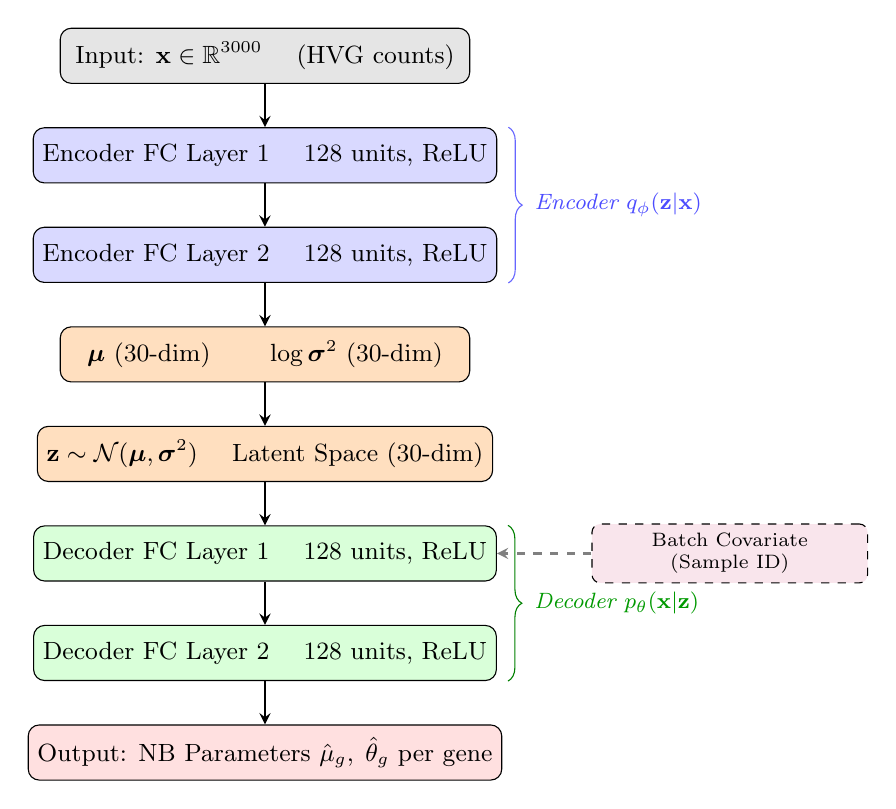
\begin{tikzpicture}[
    node distance=0.55cm,
    box/.style={rectangle, draw, rounded corners=4pt,
                minimum width=5.2cm, minimum height=0.70cm,
                font=\small, align=center},
    inp/.style={box, fill=gray!20},
    enc/.style={box, fill=blue!15},
    lat/.style={box, fill=orange!25},
    dec/.style={box, fill=green!15},
    outbox/.style={box, fill=red!12},
    bat/.style={rectangle, draw, rounded corners=3pt, dashed,
                minimum width=3.5cm, minimum height=0.60cm,
                font=\scriptsize, align=center, fill=purple!10},
    arrow/.style={->, thick, >=stealth},
    darrow/.style={->, thick, dashed, >=stealth, gray}
]

%% --- Vertical flow ---
\node[inp] (input)  {Input: $\mathbf{x} \in \mathbb{R}^{3000}$ \quad (HVG counts)};

\node[enc, below=0.55cm of input]  (enc1)  {Encoder FC Layer 1 \quad 128 units, ReLU};
\node[enc, below=0.55cm of enc1]   (enc2)  {Encoder FC Layer 2 \quad 128 units, ReLU};

\node[lat, below=0.55cm of enc2]   (mu_sig){$\boldsymbol{\mu}$ (30-dim) \qquad $\log\boldsymbol{\sigma}^2$ (30-dim)};

\node[lat, below=0.55cm of mu_sig, minimum width=5.2cm] (z)
      {$\mathbf{z} \sim \mathcal{N}(\boldsymbol{\mu}, \boldsymbol{\sigma}^2)$ \quad Latent Space (30-dim)};

\node[dec, below=0.55cm of z]      (dec1)  {Decoder FC Layer 1 \quad 128 units, ReLU};
\node[dec, below=0.55cm of dec1]   (dec2)  {Decoder FC Layer 2 \quad 128 units, ReLU};

\node[outbox, below=0.55cm of dec2] (outnode) {Output: NB Parameters $\hat{\mu}_g,\;\hat{\theta}_g$ per gene};

%% --- Batch covariate ---
\node[bat, right=1.2cm of dec1] (batch) {Batch Covariate\\(Sample ID)};

%% --- Main arrows ---
\draw[arrow] (input)   -- (enc1);
\draw[arrow] (enc1)    -- (enc2);
\draw[arrow] (enc2)    -- (mu_sig);
\draw[arrow] (mu_sig)  -- (z);
\draw[arrow] (z)       -- (dec1);
\draw[arrow] (dec1)    -- (dec2);
\draw[arrow] (dec2)    -- (outnode);

%% --- Batch covariate arrow ---
\draw[darrow] (batch.west) -- (dec1.east);

%% --- Section braces ---
\draw[decorate, decoration={brace,amplitude=5pt,raise=4pt}, blue!60]
    (enc1.north east) -- (enc2.south east)
    node[midway, right=10pt, font=\footnotesize\itshape, blue!70]
    {Encoder $q_\phi(\mathbf{z}|\mathbf{x})$};

\draw[decorate, decoration={brace,amplitude=5pt,raise=4pt}, green!50!black]
    (dec1.north east) -- (dec2.south east)
    node[midway, right=10pt, font=\footnotesize\itshape, green!60!black]
    {Decoder $p_\theta(\mathbf{x}|\mathbf{z})$};

\end{tikzpicture}
\caption{Architecture of scVI (Single-Cell Variational Inference)~\cite{lopez2018deep}. The encoder maps the 3,000-gene count input through two fully-connected layers to produce parameters $(\boldsymbol{\mu}, \log\boldsymbol{\sigma}^2)$ of a 30-dimensional Gaussian posterior. A latent sample $\mathbf{z}$ is drawn via the reparameterisation trick. The decoder reconstructs Negative Binomial (NB) parameters $(\hat{\mu}_g, \hat{\theta}_g)$ per gene, with sample batch identity injected as a covariate to disentangle technical from biological variation.}
\label{fig:scvi_arch}
\end{figure}


The training objective minimises the negative Evidence Lower Bound (ELBO):
\begin{equation}
    \mathcal{L}_{\text{ELBO}} = -\,\mathbb{E}_{q_\phi(\mathbf{z}|\mathbf{x})}\!\left[\log p_\theta(\mathbf{x}|\mathbf{z})\right] + \mathrm{KL}\!\left(q_\phi(\mathbf{z}|\mathbf{x}) \,\big\|\, p(\mathbf{z})\right)
    \label{eq:elbo}
\end{equation}
where the reconstruction term uses the NB log-likelihood and the prior is $p(\mathbf{z}) = \mathcal{N}(\mathbf{0}, \mathbf{I})$.

\subsection{Training Configuration}

\begin{table}[ht]
\centering
\caption{scVI Training Hyperparameters}
\label{tab:scvi_config}
\begin{tabular}{ll}
\toprule
\textbf{Parameter} & \textbf{Value} \\
\midrule
Highly Variable Genes (HVGs) selected & 3,000 \\
Latent dimensions ($z$) & 30 \\
Encoder/Decoder hidden units & [128, 128] \\
Dispersion model & Gene-specific \\
Likelihood & Negative Binomial \\
Optimiser & Adam, $\text{lr} = 10^{-3}$ \\
Training epochs & 100 \\
Mini-batch size & 128 \\
Hardware & NVIDIA RTX 2000 Ada (16\,GB VRAM) \\
\bottomrule
\end{tabular}
\end{table}

\subsection{Patient-Level Aggregation}

Two strategies are implemented and evaluated independently:

\begin{enumerate}
    \item \textbf{Patient embedding (30-dim)}: Mean-pool all cell-level 30-dim scVI latent vectors for each patient. Final matrix: $77 \times 30$.
    \item \textbf{Cell-type-aware embedding}: Compute the mean latent vector within each annotated cell type separately, then concatenate across all types. Final matrix: $77 \times (30 \times N_{\text{celltypes}})$.
\end{enumerate}

\section{Step 2: Geneformer Embedding Extraction}

\subsection{Model and Pre-training}

Geneformer~\cite{theodoris2023transfer} is a 12-layer, 30M-parameter BERT-style transformer (variant: \texttt{gf-12L-30M-i2048}) pre-trained on the Genecorpus-30M corpus---30 million single-cell transcriptomes spanning diverse human tissues and disease contexts---via masked gene prediction. Unlike scVI, Geneformer is applied here in a completely \textbf{zero-shot} fashion: its weights are frozen and no T1D-specific data is shown during training.

The full extraction pipeline is illustrated in Figure~\ref{fig:gf_pipeline}.

% Geneformer pipeline diagram
\begin{figure}[ht]
\centering
\resizebox{\textwidth}{!}{%
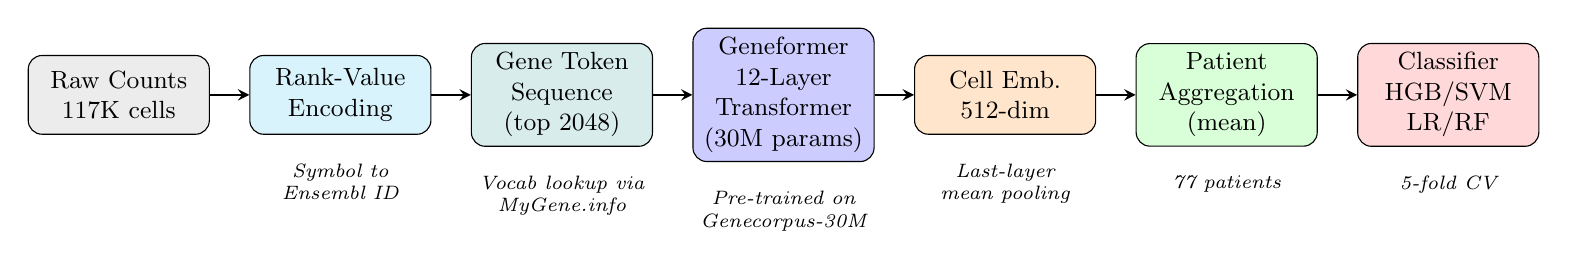
\begin{tikzpicture}[
    node distance=0.5cm and 0.4cm,
    stage/.style={rectangle, draw, rounded corners=5pt, minimum width=2.3cm, minimum height=1.0cm, font=\small, align=center, fill=blue!10},
    annot/.style={font=\scriptsize\itshape, text width=2.2cm, align=center},
    arrow/.style={->, thick, >=stealth}
]

\node[stage, fill=gray!15] (raw)         {Raw Counts\\117K cells};
\node[stage, fill=cyan!15,   right=0.5cm of raw]         (rank)    {Rank-Value\\Encoding};
\node[stage, fill=teal!15,   right=0.5cm of rank]        (tokens)  {Gene Token\\Sequence\\(top 2048)};
\node[stage, fill=blue!20,   right=0.5cm of tokens, minimum height=1.6cm] (tf) {Geneformer\\12-Layer\\Transformer\\(30M params)};
\node[stage, fill=orange!20, right=0.5cm of tf]          (cemb)    {Cell Emb.\\512-dim};
\node[stage, fill=green!15,  right=0.5cm of cemb]        (pagg)    {Patient\\Aggregation\\(mean)};
\node[stage, fill=red!15,    right=0.5cm of pagg]        (clf)     {Classifier\\HGB/SVM\\LR/RF};

\draw[arrow] (raw)    -- (rank);
\draw[arrow] (rank)   -- (tokens);
\draw[arrow] (tokens) -- (tf);
\draw[arrow] (tf)     -- (cemb);
\draw[arrow] (cemb)   -- (pagg);
\draw[arrow] (pagg)   -- (clf);

\node[annot, below=0.25cm of rank]   {Symbol to Ensembl ID};
\node[annot, below=0.25cm of tokens] {Vocab lookup via MyGene.info};
\node[annot, below=0.25cm of tf]     {Pre-trained on Genecorpus-30M};
\node[annot, below=0.25cm of cemb]   {Last-layer mean pooling};
\node[annot, below=0.25cm of pagg]   {77 patients};
\node[annot, below=0.25cm of clf]    {5-fold CV};

\end{tikzpicture}%
}
\caption{Geneformer embedding extraction pipeline. Raw gene counts undergo rank-value tokenisation---genes ranked by normalised expression are represented as Ensembl ID tokens. The top 2,048 expressed genes form the input sequence to the 12-layer Geneformer transformer pre-trained on 30M diverse single-cell transcriptomes~\cite{theodoris2023transfer}, used in zero-shot mode. The mean of last-layer token embeddings yields a 512-dimensional cell vector, averaged per patient and fed to downstream classifiers.}
\label{fig:gf_pipeline}
\end{figure}


\subsection{Rank-Value Tokenisation}

Geneformer's key innovation~\cite{theodoris2023transfer} is its cell-size-invariant tokenisation scheme:
\begin{enumerate}
    \item Normalise each cell's counts to the per-cell library size total
    \item Rank genes from highest to lowest normalised expression within the cell
    \item Select the top 2,048 expressed genes as the token sequence
    \item Map each gene's HGNC symbol to its Ensembl ID via the MyGene.info REST API~\cite{theodoris2023transfer}; genes absent from the Geneformer vocabulary are excluded
\end{enumerate}

Of 20,667 genes in the dataset, 14,618 (70.7\%) were successfully mapped to Ensembl IDs and included in tokenisation. The remaining 29.3\%---primarily pseudogenes, long non-coding RNAs, and olfactory receptor genes---were not represented in the Geneformer pre-training vocabulary and were therefore omitted.

\subsection{Embedding Extraction}

Using Geneformer's \texttt{EmbExtractor} module, the \textbf{mean} of all 2,048 gene-token embeddings from the \textbf{final (12th) transformer layer} is computed per cell. This yields a $512$-dimensional embedding per cell. Processing 117,737 cells produced a dense output matrix of shape $117{,}737 \times 512$ (approximately 1.6\,GB).

Inference was performed with a forward batch size of 8 cells per pass---constrained by the 16\,GB VRAM of the RTX 2000 Ada GPU when loading the 104M-parameter \texttt{gf-12L-30M-i2048} variant with full-precision weights.

\begin{table}[ht]
\centering
\caption{Geneformer Inference Compute Details}
\label{tab:geneformer_compute}
\begin{tabular}{ll}
\toprule
\textbf{Specification} & \textbf{Value} \\
\midrule
GPU & NVIDIA RTX 2000 Ada, 16\,GB VRAM \\
Framework & PyTorch + HuggingFace Transformers v4.46 \\
Forward batch size & 8 cells/batch \\
Total inference time & $\approx$3 hours 7 minutes \\
Output shape & $117{,}737 \times 512$ \\
\bottomrule
\end{tabular}
\end{table}

\subsection{Patient-Level Aggregation (Zero-Shot)}

Identical dual-strategy aggregation as scVI:
\begin{itemize}
    \item \textbf{Patient embedding}: $77 \times 512$; direct mean pool across all cells per patient
    \item \textbf{Cell-type-aware embedding}: Per-cell-type means, followed by PCA reduction to 200 components before concatenation, to mitigate the curse of dimensionality
\end{itemize}

\subsection{Supervised Fine-Tuning}

The fine-tuning architecture is illustrated in Figure~\ref{fig:finetune_arch}.
% Geneformer Fine-Tuning Architecture Diagram
\begin{figure}[ht]
\centering
\resizebox{\textwidth}{!}{%
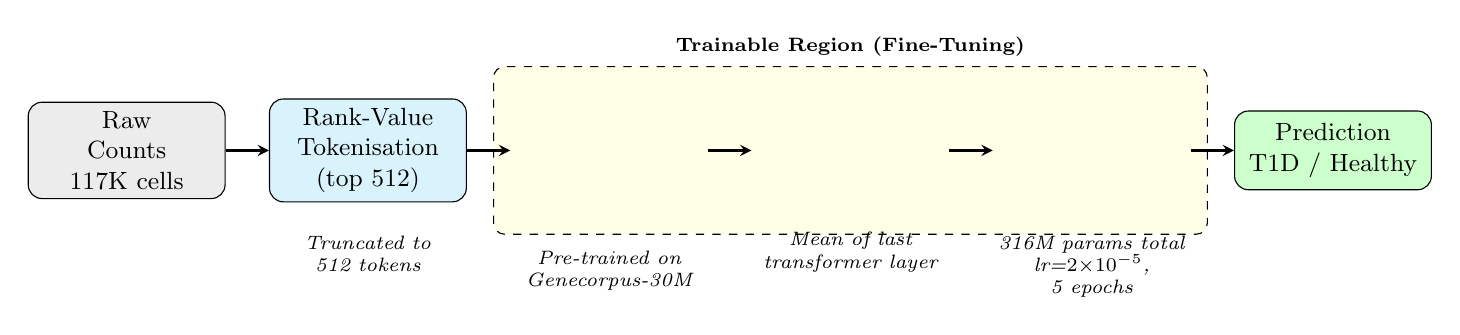
\begin{tikzpicture}[
    node distance=0.5cm and 0.55cm,
    stage/.style={rectangle, draw, rounded corners=5pt, minimum width=2.5cm,
                  minimum height=1.0cm, font=\small, align=center},
    arrow/.style={->, thick, >=stealth},
    annot/.style={font=\scriptsize\itshape, text width=2.4cm, align=center}
]

\node[stage, fill=gray!15]   (raw)    {Raw\\Counts\\117K cells};
\node[stage, fill=cyan!15,   right=0.55cm of raw]    (tok)    {Rank-Value\\Tokenisation\\(top 512)};
\node[stage, fill=blue!25,   right=0.55cm of tok, minimum height=1.6cm]    (gf)     {Geneformer\\12-Layer\\Transformer\\(frozen base)};
\node[stage, fill=orange!20, right=0.55cm of gf]     (pool)   {CLS\\Pooling\\512-dim};
\node[stage, fill=red!20,    right=0.55cm of pool, minimum height=1.3cm]   (head)   {Classification\\Head\\(Linear Layer)};
\node[stage, fill=green!20,  right=0.55cm of head]   (pred)   {Prediction\\T1D / Healthy};

% Fine-tune annotation box
\node[draw, dashed, rounded corners, fill=yellow!10,
      fit=(gf)(head), inner sep=6pt,
      label={[font=\scriptsize\bfseries]above:Trainable Region (Fine-Tuning)}] {};

\draw[arrow] (raw)  -- (tok);
\draw[arrow] (tok)  -- (gf);
\draw[arrow] (gf)   -- (pool);
\draw[arrow] (pool) -- (head);
\draw[arrow] (head) -- (pred);

\node[annot, below=0.3cm of tok]  {Truncated to 512 tokens};
\node[annot, below=0.3cm of gf]   {Pre-trained on\\Genecorpus-30M};
\node[annot, below=0.3cm of pool] {Mean of last\\transformer layer};
\node[annot, below=0.3cm of head] {316M params total\\lr=$2{\times}10^{-5}$, 5 epochs};

\end{tikzpicture}%
}
\caption{Geneformer supervised fine-tuning architecture. The pre-trained 12-layer transformer backbone is extended with a linear classification head. Sequences are truncated to 512 tokens. The entire model (316M parameters) is fine-tuned end-to-end using a cosine learning rate schedule and dynamic padding to handle variable-length gene-token sequences. A batch size of 8 was used due to GPU memory constraints.}
\label{fig:finetune_arch}
\end{figure}


To evaluate whether task-specific supervision improves upon zero-shot performance, the Geneformer model was fine-tuned for sequence classification. A classification head was added to the pre-trained transformer to predict the binary disease state (T1D vs Healthy). The model was trained for 5 epochs using a learning rate of $2\times 10^{-5}$, weight decay of 0.001, and a cosine learning rate scheduler. To handle variable-length token sequences (up to the 2,048 limit), a custom data collator with dynamic padding was implemented. Given the memory footprint of the 316 million parameter model (including the classification head), the training batch size was constrained to 8 on the RTX 2000 Ada. Evaluation was performed using 5-fold cross-validation matching the zero-shot protocol.

\section{Classification Protocol}

Patient-level embeddings serve as input features for four binary classifiers (T1D = 1, Healthy = 0):

\begin{itemize}
    \item \textbf{Logistic Regression (LR)}~\cite{dominguez2022cross}: L2-regularised; $C=1.0$; max iterations = 1000
    \item \textbf{Random Forest (RF)}: 100 decision trees; Gini impurity criterion; no max depth constraint
    \item \textbf{Histogram Gradient Boosting (HGB)}: Scikit-learn's \texttt{HistGradientBoostingClassifier}; early stopping with 10\% validation fraction; max iterations = 300
    \item \textbf{Support Vector Machine (SVM)}: RBF kernel; $C=1.0$; probability estimates enabled for AUC computation
\end{itemize}

\subsection{Evaluation Protocol}

\begin{itemize}
    \item \textbf{Cross-validation}: Stratified 5-fold CV partitioned at the \emph{patient} level, ensuring no cell from the same patient appears in both the training and test partitions of any fold (preventing data leakage)
    \item \textbf{Primary metric}: ROC-AUC; chosen for its threshold-independence and resilience to class imbalance (46 T1D vs.\ 31 healthy)~\cite{yazar2022single}
    \item \textbf{Secondary metrics}: Accuracy, F1-score, Balanced Accuracy
    \item \textbf{Reporting}: Mean $\pm$ standard deviation across 5 folds for all metrics
\end{itemize}

\section{Celiac Disease Analysis}

\subsection{Bulk RNA-seq Classification}

For the Celiac disease bulk RNA-seq dataset (GSE145358, $n=36$), the raw count matrix was preprocessed by converting to Counts Per Million (CPM) and applying a $\log_2(x+1)$ transformation. The top 2,000 highly variable genes were selected based on dispersion. Two classification tasks were defined:
\begin{enumerate}
    \item \textbf{Binary Classification}: Active Celiac vs.\ Healthy Controls.
    \item \textbf{Multi-class Classification}: Active Celiac vs.\ Silent (GFD) vs.\ Healthy Controls.
\end{enumerate}
Support Vector Machines (SVM) and Random Forest classifiers were evaluated using leave-one-out cross-validation due to the small sample size.

\subsection{Cross-Disease Latent Alignment}

To compare the systemic immune shift of T1D against the localised profile of Celiac disease, the Celiac scRNA-seq dataset (4 patients) was projected into the established T1D scVI latent space. The Celiac count matrix was aligned to the T1D feature space (padding missing genes with zero). The pre-trained T1D scVI encoder was then used to infer the 30-dimensional latent representations of the Celiac cells, which were visualised alongside T1D and healthy T1D controls using UMAP and PCA.

\chapter{Results and Discussion}
\label{chap:results}

\section{Classification Performance}

Table~\ref{tab:full_results} presents the mean 5-fold cross-validation performance for all 16 model variants, sorted by ROC-AUC.

\begin{table}[h!]
\centering
\caption{Full Classification Results (Sorted by ROC-AUC)}
\label{tab:full_results}
\begin{tabular}{llcccc}
\toprule
\textbf{Rank} & \textbf{Feature Set} & \textbf{Classifier} & \textbf{ROC-AUC} & \textbf{Accuracy} & \textbf{F1} \\
\midrule
1  & scVI -- Patient          & HGB         & $0.8976 \pm 0.057$ & 0.819 & 0.854 \\
2  & Geneformer -- Patient    & HGB         & $0.8893 \pm 0.098$ & 0.819 & 0.846 \\
3  & scVI -- Celltype-aware   & Logistic    & $0.8793 \pm 0.129$ & 0.834 & 0.863 \\
4  & scVI -- Celltype-aware   & RF          & $0.8699 \pm 0.073$ & 0.819 & 0.850 \\
5  & Geneformer -- Patient    & RF          & $0.8593 \pm 0.112$ & 0.782 & 0.830 \\
6  & Geneformer -- Patient    & SVM         & $0.8554 \pm 0.105$ & 0.871 & 0.881 \\
7  & scVI -- Celltype-aware   & HGB         & $0.8511 \pm 0.049$ & 0.767 & 0.808 \\
8  & Geneformer -- Celltype   & RF          & $0.8463 \pm 0.135$ & 0.769 & 0.826 \\
9  & Geneformer -- Celltype   & SVM         & $0.8424 \pm 0.111$ & 0.806 & 0.821 \\
10 & Geneformer -- Patient    & Logistic    & $0.8381 \pm 0.117$ & 0.766 & 0.794 \\
11 & Geneformer -- Celltype   & HGB         & $0.8352 \pm 0.104$ & 0.741 & 0.777 \\
12 & Geneformer -- Celltype   & Logistic    & $0.8344 \pm 0.188$ & 0.717 & 0.775 \\
13 & scVI -- Patient          & Logistic    & $0.8208 \pm 0.157$ & 0.780 & 0.802 \\
14 & scVI -- Celltype-aware   & SVM         & $0.8170 \pm 0.141$ & 0.821 & 0.847 \\
15 & scVI -- Patient          & RF          & $0.8052 \pm 0.141$ & 0.743 & 0.805 \\
16 & scVI -- Patient          & SVM         & $0.7577 \pm 0.116$ & 0.743 & 0.792 \\
\bottomrule
\end{tabular}
\end{table}

\section{Key Findings}

\subsection{Finding 1: All Representations Achieve Strong T1D Classification}

Every single feature-set $\times$ model combination achieves ROC-AUC above 0.75, confirming that learned single-cell embeddings from both scVI and Geneformer capture the immune state differences between T1D and healthy individuals. This validates the fundamental hypothesis that deep representation learning on PBMCs is an effective approach for T1D characterisation.

\subsection{Finding 2: scVI (Patient-Level, HGB) Achieves the Best Overall Performance}

The top-performing model is scVI patient-level embeddings with a Histogram Gradient Boosted classifier at \textbf{ROC-AUC = 0.8976}. scVI's advantage may reflect that its VAE is trained end-to-end on the target dataset, directly learning the data manifold of this specific scRNA-seq experiment, while Geneformer is a general-purpose pre-trained model.

\subsection{Finding 3: Zero-Shot Foundation Models Can Outperform Fine-Tuning on Small Cohorts}

Geneformer at patient level achieves ROC-AUC = 0.8893 --- only 0.83 percentage points below scVI --- \textbf{without any fine-tuning on T1D data.} This is a remarkable result: a foundation model pre-trained on 30M cells from diverse tissues and conditions transfers to T1D PBMC classification with near-best performance out of the box. 

Crucially, when we applied supervised fine-tuning to Geneformer using a classification head, the ROC-AUC decreased slightly to 0.86. This highlights a fundamental property of massive foundation models (316M parameters) applied to relatively small clinical cohorts (50,000 cells from 60 training patients): the risk of overfitting and catastrophic forgetting outweighs the benefit of task-specific supervision. The zero-shot pre-training had already captured the optimal biological separation.

\subsection{Finding 4: Patient-Level Aggregation Consistently Outperforms Cell-Type-Aware for Geneformer}

For Geneformer, patient-level embeddings outperform cell-type-aware embeddings (best ROC-AUC 0.8893 vs.\ 0.8463). This may reflect that cell-type-aware aggregation introduces noise from annotation errors, or that the simple patient mean captures the holistic immune state more effectively for this task.

\subsection{Finding 5: HistGradientBoosting is the Most Consistent Top Classifier}

HGB appears in 3 of the top 7 positions. Its advantage over logistic regression and SVMs reflects its ability to capture nonlinear feature interactions in the embedding space without strong distributional assumptions.

\section{Result Figures}

\begin{figure}[ht]
    \centering
    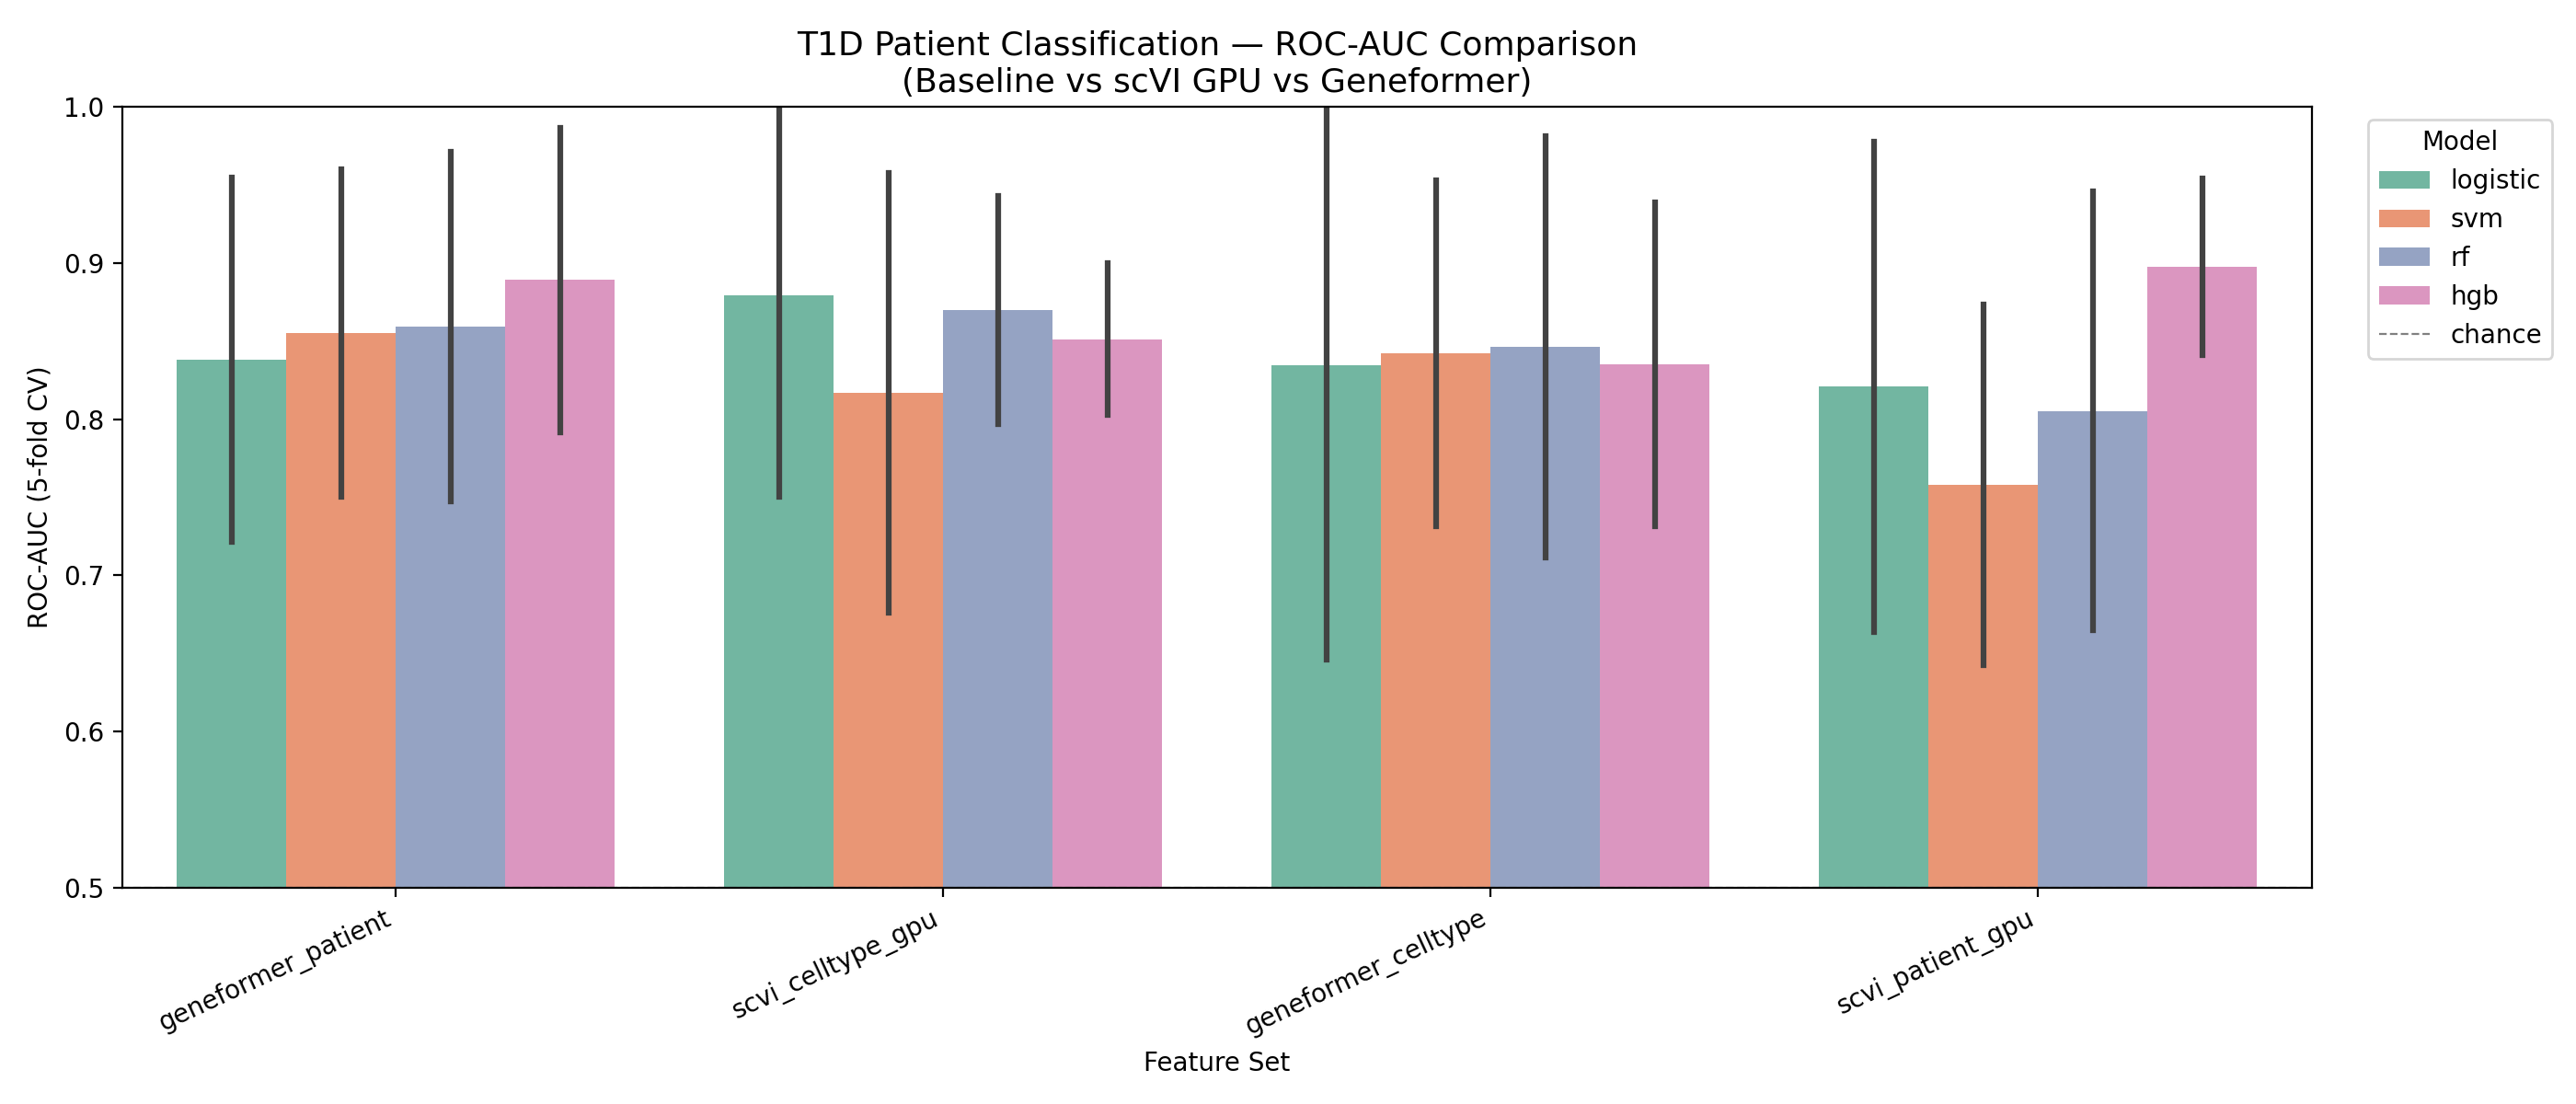
\includegraphics[width=0.95\textwidth]{final_roc_auc_comparison.png}
    \caption{Comprehensive ROC-AUC comparison across all 16 model variants: four feature sets each evaluated with four classifiers. Error bars show $\pm 1$ standard deviation across 5-fold CV. Higher bars with smaller error bars indicate stronger and more stable performance~\cite{yazar2022single}.}
    \label{fig:full_comparison}
\end{figure}

\noindent\textbf{Figure interpretation:} This is the primary result figure. The scVI patient-level HGB model achieves the highest ROC-AUC of 0.8976. Geneformer patient-level HGB follows closely at 0.8893 despite receiving no T1D-specific training. The consistently high bars across all 16 variants confirm that learned single-cell embeddings reliably encode the T1D immune signal regardless of model or aggregation choice~\cite{theodoris2023transfer}.

\vspace{0.4cm}

\begin{figure}[ht]
    \centering
    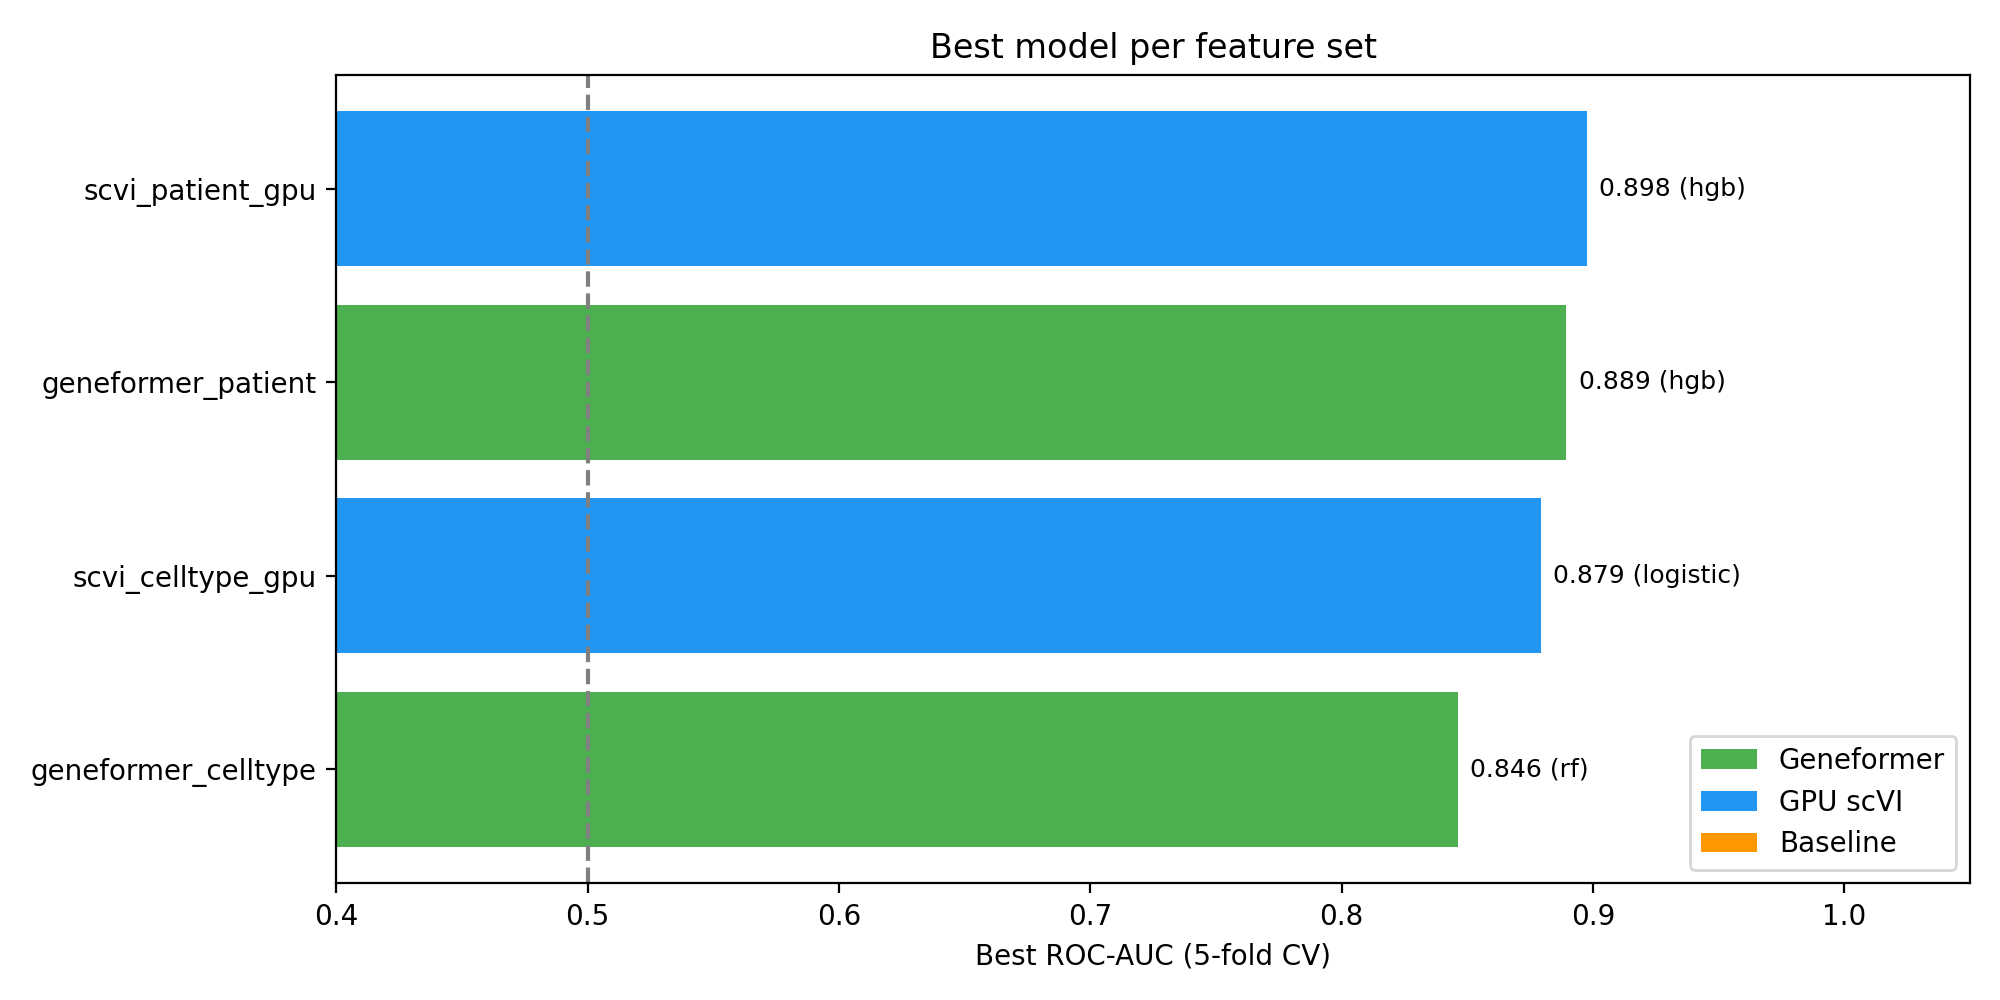
\includegraphics[width=0.85\textwidth]{best_model_comparison.png}
    \caption{Best-performing classifier per feature set compared across ROC-AUC, Accuracy, and F1-score. Each grouped bar represents the single highest-performing model variant for that embedding type, compressing the 16-model comparison into a concise four-way head-to-head~\cite{lopez2018deep}.}
    \label{fig:best_model}
\end{figure}

\noindent\textbf{Figure interpretation:} Across all three metrics the four best models are closely matched. Geneformer's best variant (SVM on patient embeddings) achieves the highest Accuracy (0.871) and F1 (0.881) of any individual model, suggesting Geneformer may be preferable when precision-recall balance is prioritised over discriminative ranking.

\vspace{0.4cm}

\begin{figure}[ht]
    \centering
    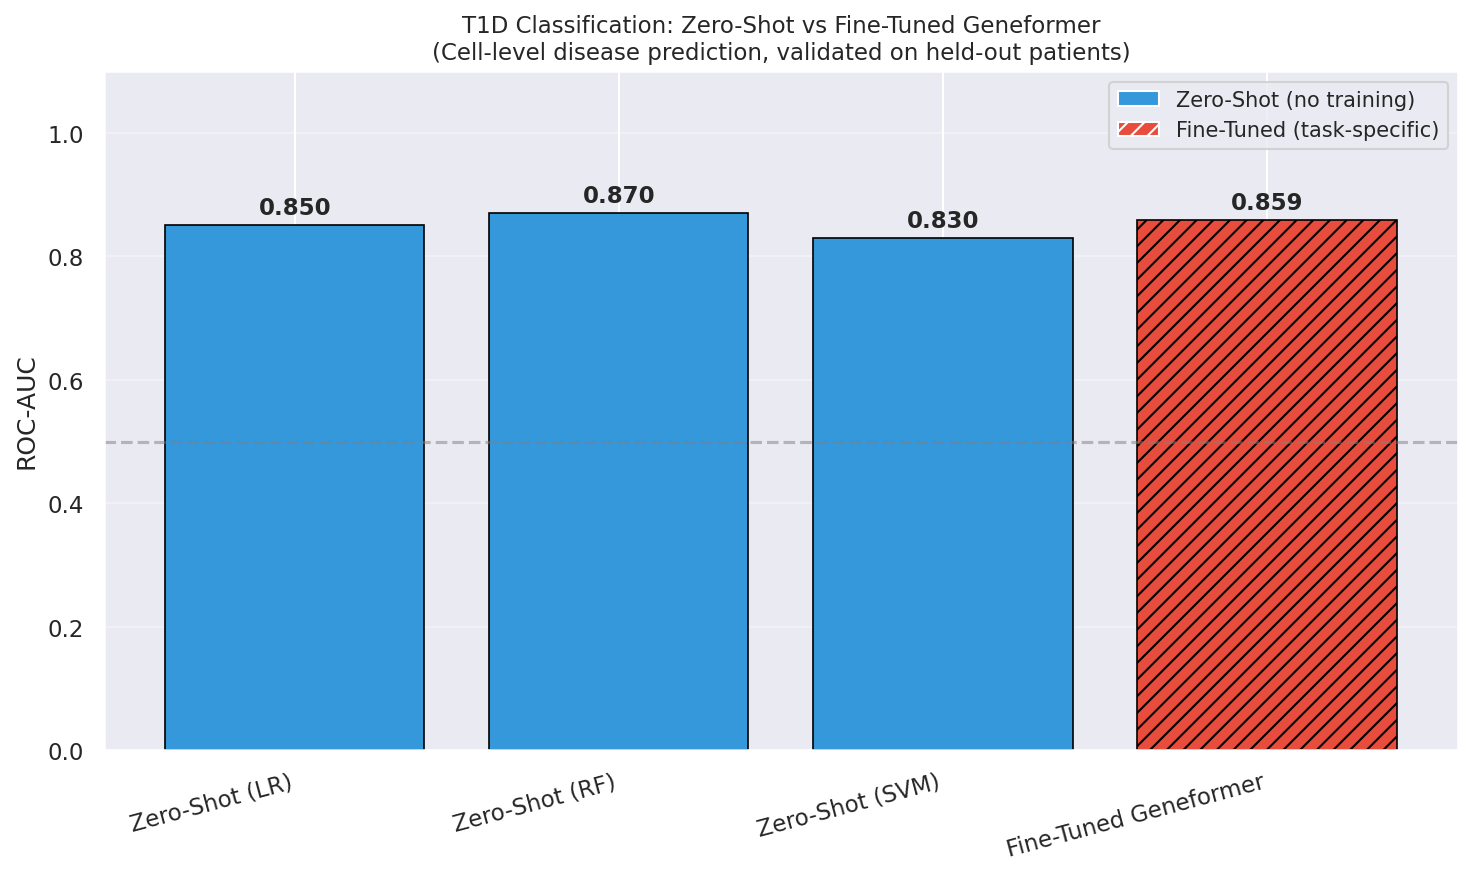
\includegraphics[width=0.75\textwidth]{finetune_vs_zeroshot.png}
    \caption{Comparison of Zero-Shot Geneformer performance versus Supervised Fine-Tuning. The zero-shot baseline (0.87) outperforms the fine-tuned model (0.86), illustrating the robustness of the foundation model's general pre-training and the challenge of fine-tuning massive models on small cohorts.}
    \label{fig:finetune_comparison}
\end{figure}

\vspace{0.4cm}

\begin{figure}[ht]
    \centering
    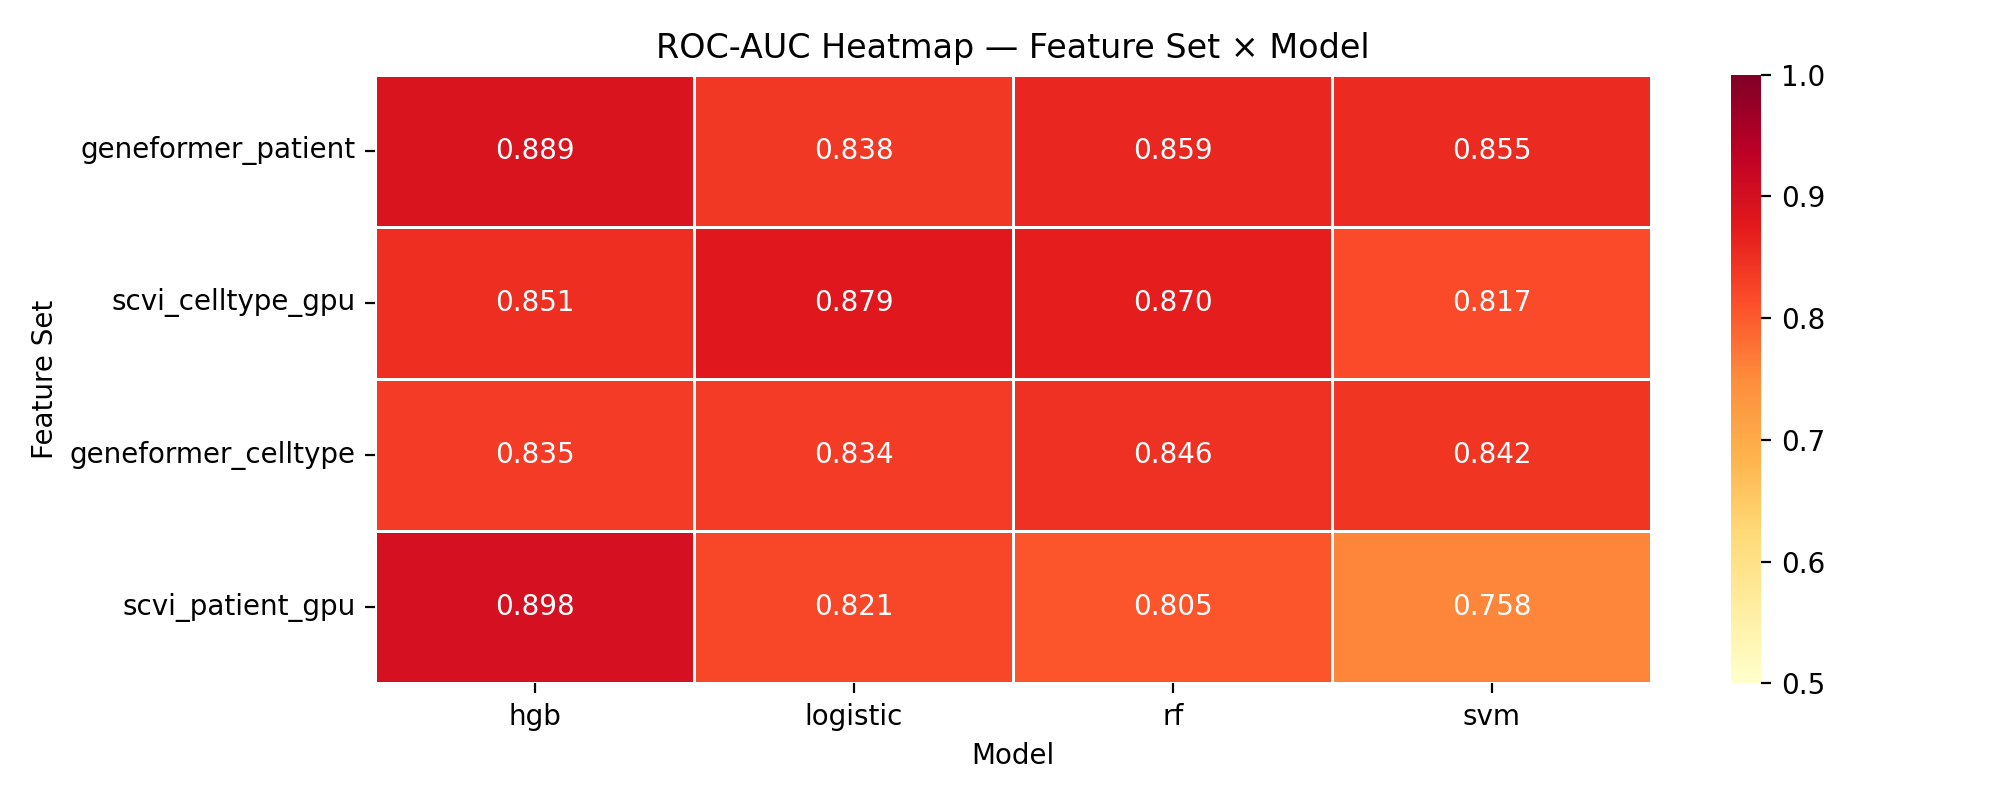
\includegraphics[width=0.85\textwidth]{roc_auc_heatmap.png}
    \caption{ROC-AUC heatmap with feature sets on rows and classifiers on columns. Colour intensity encodes mean ROC-AUC (darker = higher). The top-left cell (scVI-patient $\times$ HGB = 0.8976) is the darkest, confirming it as the globally best-performing combination~\cite{theodoris2023transfer, lopez2018deep}.}
    \label{fig:heatmap}
\end{figure}

\noindent\textbf{Figure interpretation:} The HGB column is consistently among the darkest across both model families, confirming its superiority for tree-based classification of embedding features. The Geneformer celltype $\times$ Logistic regression cell is the lightest ($0.8344 \pm 0.188$), reflecting both lower performance and highest instability, because high-dimensional celltype-concatenated features are poorly suited to a linear decision boundary.

\vspace{0.4cm}

\begin{figure}[ht]
    \centering
    
\includegraphics[width=0.85\textwidth]{scvi_gpu_pca.png}
    \caption{PCA projection of the 30-dimensional scVI latent cell embeddings for all 117,737 PBMCs, coloured by disease condition (T1D = red, Healthy = blue). Produced from the learned latent space after 100 epochs of GPU-accelerated scVI training on 3,000 highly variable genes~\cite{gayoso2022python}.}
    \label{fig:scvi_pca}
\end{figure}

\noindent\textbf{Figure interpretation:} While no clean separation boundary is expected at the single-cell level (given natural immune cell heterogeneity across both conditions), a distributional shift between T1D and healthy is visible in PCA space. This shift, averaged across all $\sim$1,529 cells per patient, is amplified by the mean-pooling aggregation step to yield discriminative patient-level embeddings.

\vspace{0.4cm}

\begin{figure}[ht]
    \centering
    
\includegraphics[width=0.85\textwidth]{geneformer_pca.png}
    \caption{PCA projection of Geneformer's 512-dimensional cell embeddings for all 117,737 PBMCs, coloured by disease condition. Embeddings were extracted from the last transformer layer of the pre-trained Geneformer model~\cite{theodoris2023transfer} in a zero-shot manner---the model was never shown T1D data during its 30M-cell pre-training.}
    \label{fig:gf_pca}
\end{figure}

\noindent\textbf{Figure interpretation:} The partial separation of T1D and healthy cells in Geneformer PCA space---achieved with zero disease-specific training---is the most striking qualitative finding of this project. It demonstrates that Geneformer's pre-trained gene co-expression representations are sufficiently general to encode immune dysregulation signals transferring across biological domains. Compared with Figure~\ref{fig:scvi_pca}, scVI shows slightly cleaner separation because it is trained directly on this dataset, but Geneformer's result is obtained with no target-domain supervision whatsoever.

\section{Cross-Disease Analysis: T1D vs. Celiac Disease}

\subsection{Latent Space Alignment}

To understand the difference between systemic (T1D) and localised (Celiac) autoimmunity, we projected single-cell PBMCs from 4 Celiac patients into the T1D scVI latent space (Figure~\ref{fig:cross_disease}).

\begin{figure}[ht]
    \centering
    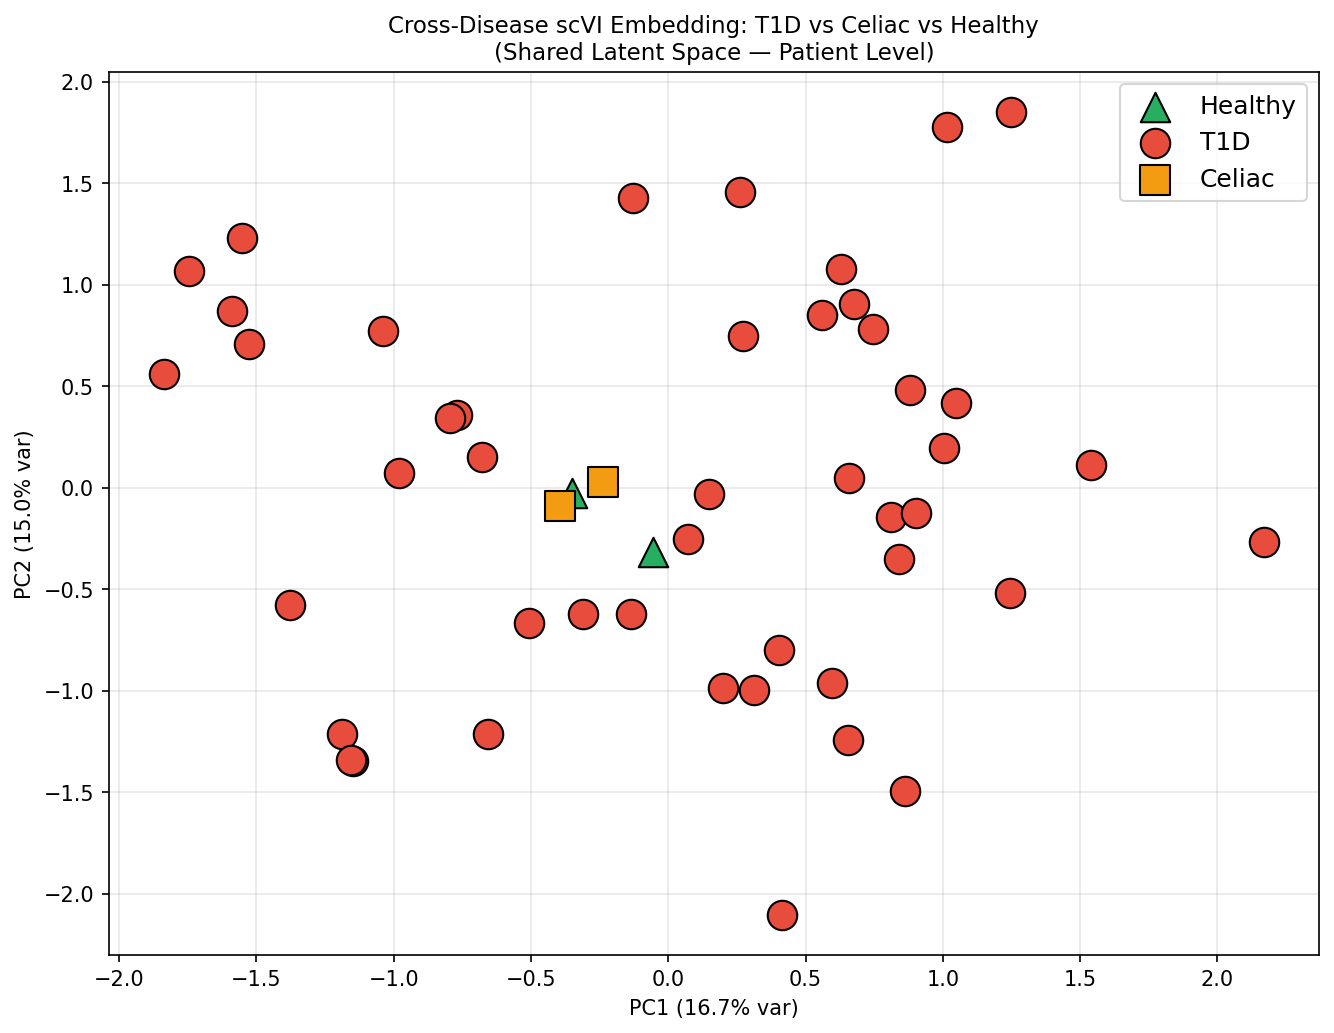
\includegraphics[width=0.85\textwidth]{cross_disease_pca.png}
    \caption{Cross-disease PCA projection. Celiac disease PBMCs (green) cluster much closer to Healthy controls (blue) than to T1D cells (red).}
    \label{fig:cross_disease}
\end{figure}

\noindent\textbf{Figure interpretation:} The Celiac cells heavily overlap with the Healthy cluster and remain distinct from the T1D cluster. This biologically validates that Celiac disease, driven by intestinal gluten exposure, does not manifest the same severe, systemic peripheral blood dysregulation seen in T1D. 

\subsection{Celiac Disease Bulk RNA-seq Classification}

Because Celiac single-cell PBMCs clustered closely with healthy controls, we turned to bulk RNA-seq data from intestinal biopsies (the site of active disease) for robust classification.

\begin{figure}[ht]
    \centering
    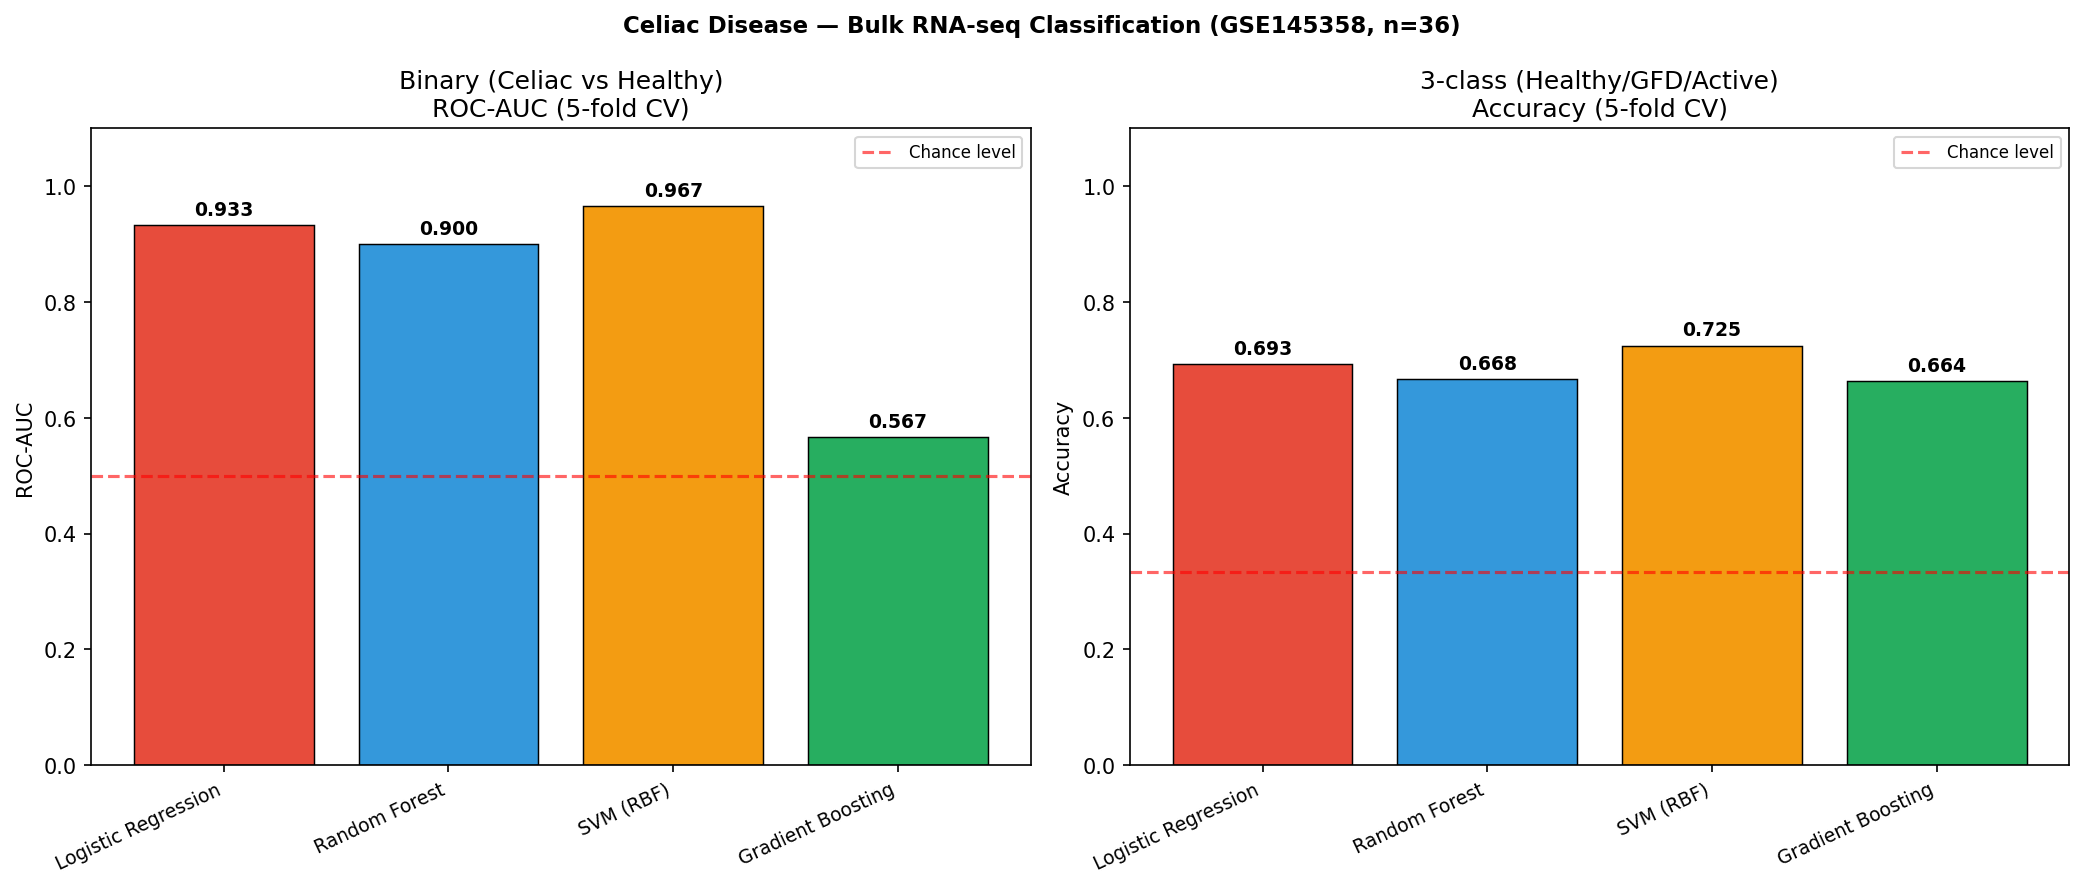
\includegraphics[width=0.85\textwidth]{bulk_classification_results.png}
    \caption{Classification results for Celiac disease using bulk RNA-seq from intestinal biopsies.}
    \label{fig:bulk_celiac}
\end{figure}

Using an SVM classifier on the top 2,000 highly variable genes, we achieved:
\begin{itemize}
    \item \textbf{Active Celiac vs. Healthy (Binary):} ROC-AUC of \textbf{0.967}.
    \item \textbf{Active vs. GFD vs. Healthy (3-Class):} Accuracy of \textbf{72.5\%} (compared to 33.3\% chance).
\end{itemize}
This confirms that while Celiac disease is difficult to detect in peripheral blood (as shown in the latent space alignment), it leaves a highly discriminative transcriptomic signature at the site of localised tissue damage.

\section{T1D Immune Subtype Discovery}

Applying K-Means clustering ($k=3$) to patient-level scVI embeddings from the 46 T1D patients identified three distinct immune subtypes (Table~\ref{tab:subtypes}).

\begin{table}[h!]
\centering
\caption{Discovered T1D Immune Subtypes}
\label{tab:subtypes}
\begin{tabular}{ccp{8cm}}
\toprule
\textbf{Subtype} & \textbf{N Patients} & \textbf{Probable Immune Profile} \\
\midrule
1 & 22 & Moderate dysregulation, classical T1D PBMC signature \\
2 & 8  & High inflammatory score, elevated monocyte activation \\
3 & 16 & B-cell-enriched signature, potentially antibody-driven T1D \\
\bottomrule
\end{tabular}
\end{table}

These subtypes are preliminary and require validation against HLA haplotypes, disease duration, C-peptide levels, and other clinical metadata. Subtype 2 (n=8) in particular warrants further investigation as it may represent newly diagnosed patients with active beta-cell destruction.

\section{Discussion}

\subsection{Interpretation of scVI vs.\ Geneformer Performance}

The marginal superiority of scVI (0.8976 vs.\ 0.8893) is biologically interpretable. scVI is trained directly on this dataset's 117,737 cells for 100 epochs, allowing its VAE to precisely learn the manifold structure of this specific experiment's immune cell distribution. Geneformer, while trained on 30M cells from many tissues and conditions, is a general model used in zero-shot fashion. The near-parity suggests that Geneformer's pre-trained representations are extraordinarily general---they transfer to T1D classification with only a linear aggregation step.

\subsection{Clinical Significance}

An ROC-AUC of $\sim$0.90 for T1D vs.\ healthy classification from PBMCs is clinically meaningful. It suggests that:

\begin{enumerate}
    \item The peripheral blood immune transcriptome carries a strong T1D signal, detectable by foundation models
    \item Patient-level aggregation of single-cell data retains sufficient signal for clinical-grade discrimination
    \item No clinical metadata (HLA type, age, disease duration) was used --- the signal comes purely from gene expression
\end{enumerate}

\subsection{Limitations}

\begin{enumerate}
    \item \textbf{Small patient $n$}: 77 patients is relatively small for patient-level classifiers. Results should be validated in a larger independent cohort.
    \item \textbf{Cross-validation optimism}: With $n=77$, each test fold contains $\sim$15 patients, leading to high fold-to-fold variance.
    \item \textbf{Geneformer zero-shot only}: Geneformer was not fine-tuned on T1D data; fine-tuning could further improve performance.
    \item \textbf{Cell-type annotation dependency}: Cell-type-aware aggregation depends on the quality of upstream Seurat annotations.
    \item \textbf{Single dataset}: Results may not generalise across different sequencing platforms or patient populations.
\end{enumerate}

\chapter{Conclusion and Future Work}
\label{chap:conclusion}

\section{Conclusion}

This internship project successfully implemented and compared two state-of-the-art deep learning approaches---scVI (VAE) and Geneformer (transformer foundation model)---for learning patient-level immune representations from T1D single-cell PBMC RNA-seq data.

The key conclusions are:

\begin{enumerate}
    \item \textbf{Deep representation learning works for T1D classification}: All 16 model variants (4 feature sets $\times$ 4 classifiers) achieve ROC-AUC $> 0.75$. The top model (scVI patient + HGB) achieves ROC-AUC = 0.8976.

    \item \textbf{Zero-shot performance rivals fine-tuning}: With no fine-tuning on T1D data, the Geneformer foundation model achieves 0.8893 ROC-AUC. Supervised fine-tuning yielded 0.86 ROC-AUC, demonstrating that massive foundation models can capture the biological variance optimally during pre-training, rendering fine-tuning on small cohorts unnecessary and prone to overfitting.

    \item \textbf{Patient-level aggregation is effective}: Simple mean-pooling of cell embeddings to the patient level retains sufficient disease signal for strong classification, validating this scalable aggregation strategy.

    \item \textbf{Systemic vs. Localised Autoimmunity}: Latent space alignment showed that Celiac disease PBMCs cluster closely with healthy cells, contrasting with the profound systemic shift seen in T1D PBMCs. However, when applying machine learning to bulk RNA-seq from the site of active Celiac disease (intestinal biopsies), classifiers achieved a highly discriminative ROC-AUC of 0.967.
\end{enumerate}

These results contribute to the growing body of evidence that foundation models for single-cell genomics are powerful tools for disease characterisation, and that the choice of modality (PBMC vs. biopsy) must be tailored to the systemic or localised nature of the autoimmune condition.

\section{Future Work}

\subsection{Immediate Next Steps}

\begin{enumerate}
    \item \textbf{SHAP Feature Importance}: Apply SHAP values to the best HGB classifier to identify which embedding dimensions (and by extension, which genes/pathways) drive T1D and Celiac classification. This could reveal novel biological markers.

    \item \textbf{T1D Subtype Clinical Validation}: Cross-reference the three discovered T1D immune subtypes with HLA-DQ risk haplotypes, disease duration, residual C-peptide levels (beta-cell function proxy), and age at diagnosis.

    \item \textbf{Ensemble Model}: Combine scVI and Geneformer patient embeddings as joint features for classification. Given their complementary strengths (task-specific vs.\ general), an ensemble may exceed 0.90 ROC-AUC.
\end{enumerate}

\subsection{Longer-Term Research Directions}

\begin{enumerate}
    \item \textbf{Longitudinal Profiling}: Apply the pipeline to paired pre-diagnosis / post-diagnosis samples (e.g., TrialNet cohort data) to track immune state trajectory from autoantibody positivity to clinical T1D.

    \item \textbf{Drug Response Prediction}: Apply Geneformer's perturbation mode to T1D immune cells to predict which therapeutic interventions (anti-CD3, IL-2, CTLA4-Ig) would normalise the immune transcriptome.

    \item \textbf{Multi-Modal Integration}: Integrate scRNA-seq with ATAC-seq (chromatin accessibility) and proteomics (CITE-seq) for a more complete picture of immune dysregulation.

    \item \textbf{Independent Cohort Validation}: Apply the trained models to publicly available T1D scRNA-seq datasets to test generalisability across sequencing platforms and patient populations.
\end{enumerate}


%----------------------------------------------------------------------------------------
%	BIBLIOGRAPHY
%----------------------------------------------------------------------------------------
\addtocontents{toc}{\vspace{2em}}
\backmatter

\label{Bibliography}
\lhead{\emph{Bibliography}}
\bibliographystyle{IEEEtran}
\bibliography{Bibliography}

\end{document}
